\chapter{Precipitación total}\label{cap:resultados_tp}
La precipitación asociada a ciclones extratropicales complementa al viento (Capítulo~\ref{cap:resultados_wind10}) en la caracterización estructural del sistema. A diferencia del viento, integra procesos de calor, desde la condensación estratiforme de gran escala hasta la convección embebida de mesoescala ligada a la liberación de calor latente (Sección~\ref{subsec:tb_modelos}).
Este capítulo establece la estructura espacial de la precipitación durante las fases del ciclo de vida de los ciclones extratropicales del Atlántico Sudoccidental, siguiendo la progresión metodológica del Capítulo~\ref{cap:resultados_wind10}: (i)~evolución de las distribuciones de magnitud según intensidad del vórtice y región de génesis; (ii)~localización espacial preferencial de los máximos de precipitación; y (iii)~descomposición EOF.
La Sección~\ref{sec:pdf_tp} examina las PDF de magnitud; las Secciones~\ref{subsec:kde_tp_global} y~\ref{subsec:kde_tp_p90}, la distribución espacial de los máximos (PDFe); y las Secciones~\ref{subsec:var_exp_tp}--\ref{sec:dinamica_pc1_tp}, la estructura modal vía EOF.
Los resultados se contrastan con los del campo de viento para evaluar, en el Capítulo~\ref{chap:meof}, si ambas variables comparten una organización espacial coherente.

% --- SECCIÓN PRINCIPAL: PDF DE PRECIPITACIÓN TOTAL ---

\section{Distribución de magnitudes (PDF)}\label{sec:pdf_tp}

\begin{figure}[htbp]
\centering
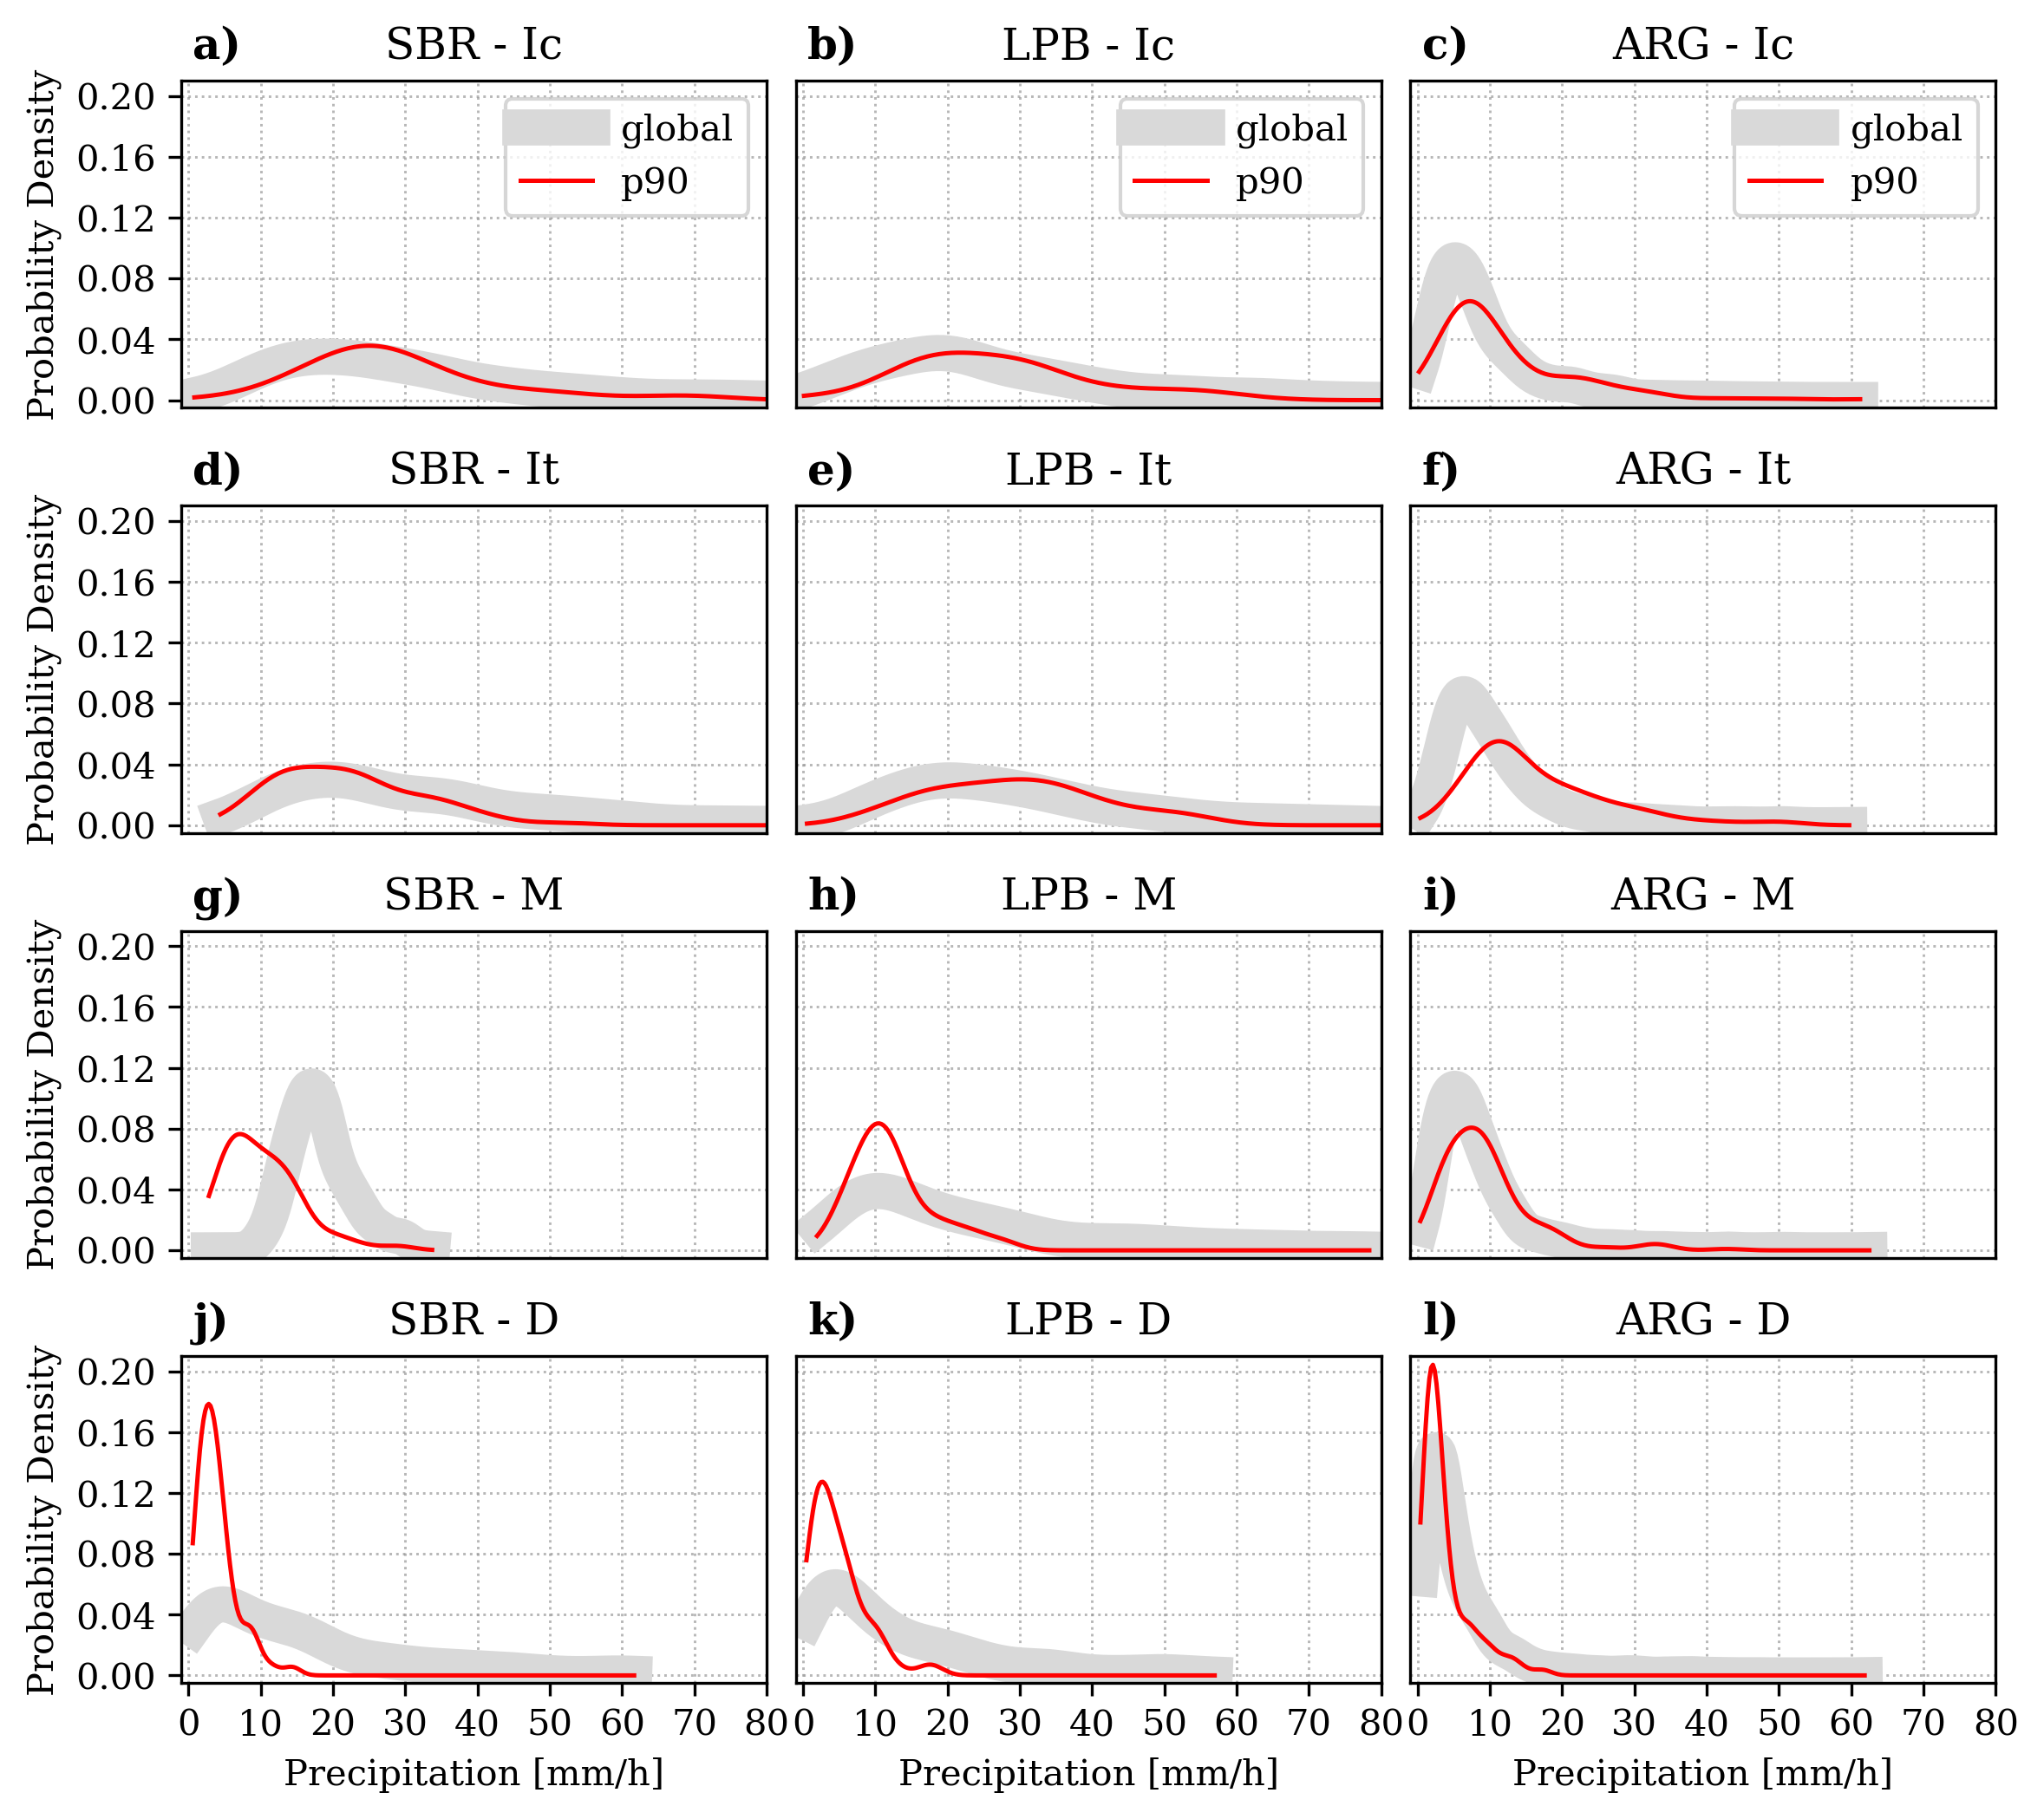
\includegraphics[width=\textwidth]{images/tp/PDF_tp_sigma025.png}
\caption[PDF de magnitudes máximas de precipitación total]{Funciones de densidad de probabilidad (PDF) para las magnitudes máximas de precipitación total (mm/h). Las columnas indican la región de ciclogénesis (SBR, LPB, ARG) y las filas la evolución a través de las fases del ciclo de vida (Ic, It, M, D). Se contrasta la Población Global (referencia, sombreado gris) con el subconjunto de los máximos de vorticidad relativa en 850 hPa alcanzados en su ciclo de vida: p90 (ciclones intensos, linea roja).}
\label{fig:pdf_tp}
\end{figure}

La Figura~\ref{fig:pdf_tp} muestra la distribución estadística de los máximos espaciales de precipitación (mm/h) para los composites del tiempo central de cada fase, estratificados por región de ciclogénesis (SBR, LPB, ARG) y por el pico de vorticidad relativa en 850 hPa alcanzado en el ciclo de vida (p90).
Como fundamentan \citet{sinclair2023relationship}, los ciclones extratropicales son la causa principal de la precipitación en estas latitudes, por lo que su escalamiento con la intensidad dinámica ayuda a caracterizar el acoplamiento entre vórtice y respuesta hidrológica.
Estos campos se extrajeron dentro del dominio lagrangiano centrado en el núcleo de cada sistema, siguiendo la metodología aplicada al viento (Capítulo~\ref{cap:resultados_wind10}).

En las fases incipiente e intensificación (paneles a--f), SBR y LPB muestran en la Población Global un perfil plano y extendido con pico modal entre 10 y 20~mm/h, reflejo de la amplia dispersión de intensidades propia de estas regiones oceánicas \citep{evans2012climatology}.
Los ciclones intensos (p90) exhiben mayores tasas, con colas que llegan a 60~mm/h y una diferenciación respecto a la Población Global que no se observa con igual claridad en ARG.
Como detallan \citet{chen2024evaluation}, la precipitación total resulta de la suma de la componente estratiforme de gran escala y la convectiva parametrizada; \citet{flaounas2018heavy} cuantifican en ciclones del Mediterráneo que la convección profunda genera las mayores tasas y controla la cola superior de la distribución, parte de ellas embebidas en la Cinta Transportadora Cálida (WCB, \textit{warm conveyor belt}).
En entornos con mayor humedad e inestabilidad estática, SBR y LPB, el desarrollo de los ciclones más intensos está ligado a mayor actividad convectiva \citep{sinclair2023relationship}. Organizada dentro del WCB, esta convección libera calor latente que intensifica el sistema \citep{blanchard2021warm} y genera precipitaciones de alta intensidad \citep{oertel2021warm}. Por ello, en los p90, el WCB es responsable de los máximos de precipitación durante las primeras fases de desarrollo.

En ARG (paneles c, f), la Población Global presenta un pico modal pronunciado en valores bajos ($\sim$5--10~mm/h, densidades $>$0.10) con caída rápida hacia valores moderados que rara vez superan los 50~mm/h, reflejo de la menor disponibilidad de humedad y la modulación orográfica de los Andes.
El subconjunto p90 durante la intensificación (panel f) muestra el pico desplazado a valores algo mayores ($\sim$10~mm/h), pero con las densidades más bajas de la fila, confirmando una menor eficiencia para concentrar precipitación extrema respecto a SBR y LPB.

Al alcanzar la madurez (paneles g--i) y el decaimiento (paneles j--l), las diferencias entre la Población Global y p90 sobresalen.
En SBR y LPB, la Población Global mantiene el pico amplio entre 15 y 20~mm/h, mientras p90 colapsa hacia la izquierda durante la madurez y, en el decaimiento, se vuelve agudo en valores mínimos (1--4~mm/h), con densidades que alcanzan 0.17 en SBR y 0.12 en LPB.
En ARG, el decaimiento (panel l) exhibe la distribución más extrema. P90 alcanza su densidad máxima absoluta ($>$0.20) en 2--5~mm/h, superando a SBR y LPB, y ambas curvas convergen a cero por encima de 15--20~mm/h; los sistemas sobre Argentina producen así precipitación casi exclusivamente en el rango de muy baja intensidad.
La disparidad en las colas se asocia a distintas forzantes regionales. \citet{yanase2014parameter} sugieren que el desarrollo ciclónico es sensible a la humedad y baroclinicidad del entorno, y \citet{gramcianinov2019properties} confirman, para el Atlántico Sur, que la combinación de baroclinicidad costera y disponibilidad de humedad determina la evolución de los sistemas.

\citet{laurila2021characteristics} señalan que los sistemas que terminan generando las rachas de viento más intensas poseen firmas dinámicas distinguibles desde etapas iniciales, mientras que la predictibilidad de la precipitación máxima resulta menor debido a su naturaleza intermitente, gobernada por la actividad frontal y la convección embebida \citep{oertel2021warm}.
En nuestro dominio, \citet{russo2025impacts} documentan, en casos representativos de SBR y el límite con LPB, flujos de calor oceánico que sostienen la baroclinicidad y anclan la convección profunda; el ensanchamiento de la Población Global se acentúa por la formación de ciclones todo el año, pues, según \citet{evans2012climatology}, el vínculo con anomalías térmicas, generadoras de humedad y estabilidad en la troposfera media, favorece la formación recurrente de ciclones con diversas estructuras térmicas en el Atlántico Sur. La energía convectiva del estrato p90 se organiza mediante fuerte advección cálida y convergencia de humedad, impulsada por la Alta Subtropical en SBR y por su interacción con el SALLJ en LPB \citep{gramcianinov2024early}.

En contraste, ARG presenta precipitaciones menores en todas las fases, reflejo de un forzamiento de latitudes altas con baja humedad absoluta y advecciones frías y secas del Pacífico sur. Como señalan \citet{gramcianinov2019properties}, los ciclones de ARG están dominados por la baroclinicidad de latitudes medias y registran menos eventos que superen los 20~mm/día, mientras que los de LPB y SBR dependen de la liberación de calor latente y concentran las tasas más intensas, con marcada similitud entre ambas. \citet{coutodesouza2024thesis} corrobora esta dualidad desde la energética atmosférica. ARG se sustenta en la cadena baroclínica clásica (Sección~\ref{subsec:tb_arg}), mientras que en LPB y SBR dominan los procesos diabáticos convectivos (Secciones~\ref{subsec:tb_sbr} y~\ref{subsec:tb_lpb}).

El desacople entre la máxima intensidad dinámica y la máxima precipitación durante la madurez confirma una relación no lineal entre vorticidad y forzantes de precipitación, consistente con climatologías del Hemisferio Sur donde el máximo de precipitación ocurre en promedio antes que el de intensidad \citep{dacre2023climatology}. \citet{heitmann2024lifecycle} cuantifica de forma independiente esta secuencia de fases para casi 5000 ciclones invernales del Atlántico Norte. El volumen de precipitación asociado al WCB alcanza su pico sistemáticamente antes de que el propio WCB alcance su intensidad máxima, la cual a su vez precede al mínimo de presión del ciclón, lo que sugiere que este desfase escalonado no es una particularidad del Atlántico Sur sino una propiedad más general de la relación entre el WCB y el ciclón que lo alberga. Los ciclones p90 evolucionan hacia sistemas profundos que agotan su acceso a la masa de aire húmedo e inestable transportada por el WCB. El núcleo experimenta entonces una intrusión seca (\textit{dry intrusion}) inducida por la fractura frontal, mediante la cual aire frío, subsidente y de baja humedad de la alta troposfera desciende al oeste del centro del sistema, consistente con la subsidencia troposférica documentada para el Hemisferio Norte por \citet{shapiro1999bridge}.

\citet{corner2025classification} cuantifica el mecanismo de retroalimentación que sostiene esta no linealidad. El calentamiento diabático de la lluvia intensa genera anomalías de vorticidad potencial que refuerzan la circulación en niveles bajos, sustentando las colas pesadas ($>$60~mm/h) de p90 en SBR y LPB durante la intensificación, antes de que el aislamiento del núcleo corte el suministro de humedad. Esto refuta que el forzamiento dinámico se traduzca en mayor lluvia extrema durante todo el ciclo de vida. En el Atlántico Sur, los ciclones con vientos más intensos tienden a secarse en su núcleo durante la madurez, de modo que las mayores tasas de p90 ocurren predominantemente en génesis e intensificación, o en sistemas de intensidad moderada con configuraciones termodinámicas más eficientes para el anclaje convectivo. Esto coincide con \citet{mcerlich2023extremes}, quienes muestran para el Hemisferio Sur que la precipitación más intensa ocurre en la profundización previa al pico de intensidad, concentrando hasta el 80\% de la precipitación total de los compuestos ciclón-centrados, con una ocurrencia que cae al 46\% de ese máximo hacia el resto del ciclo de vida.

Si la magnitud máxima se desplaza o desaparece del núcleo en las fases tardías, es necesario establecer dónde se reorganiza esa lluvia residual y si ello depende de la intensidad dinámica del sistema. La siguiente sección examina, mediante estimación de densidad espacial (PDFe), la ubicación preferencial de los máximos de precipitación en el marco lagrangiano para la Población Global.
% --- SECCIÓN PRINCIPAL: PDFe ESPACIAL DE PRECIPITACIÓN ---

\section{Distribución espacial de máximos (PDFe)}\label{sec:pdfe_tp}

\subsection{Población Global}\label{subsec:kde_tp_global}

\begin{figure}[htbp]
\centering
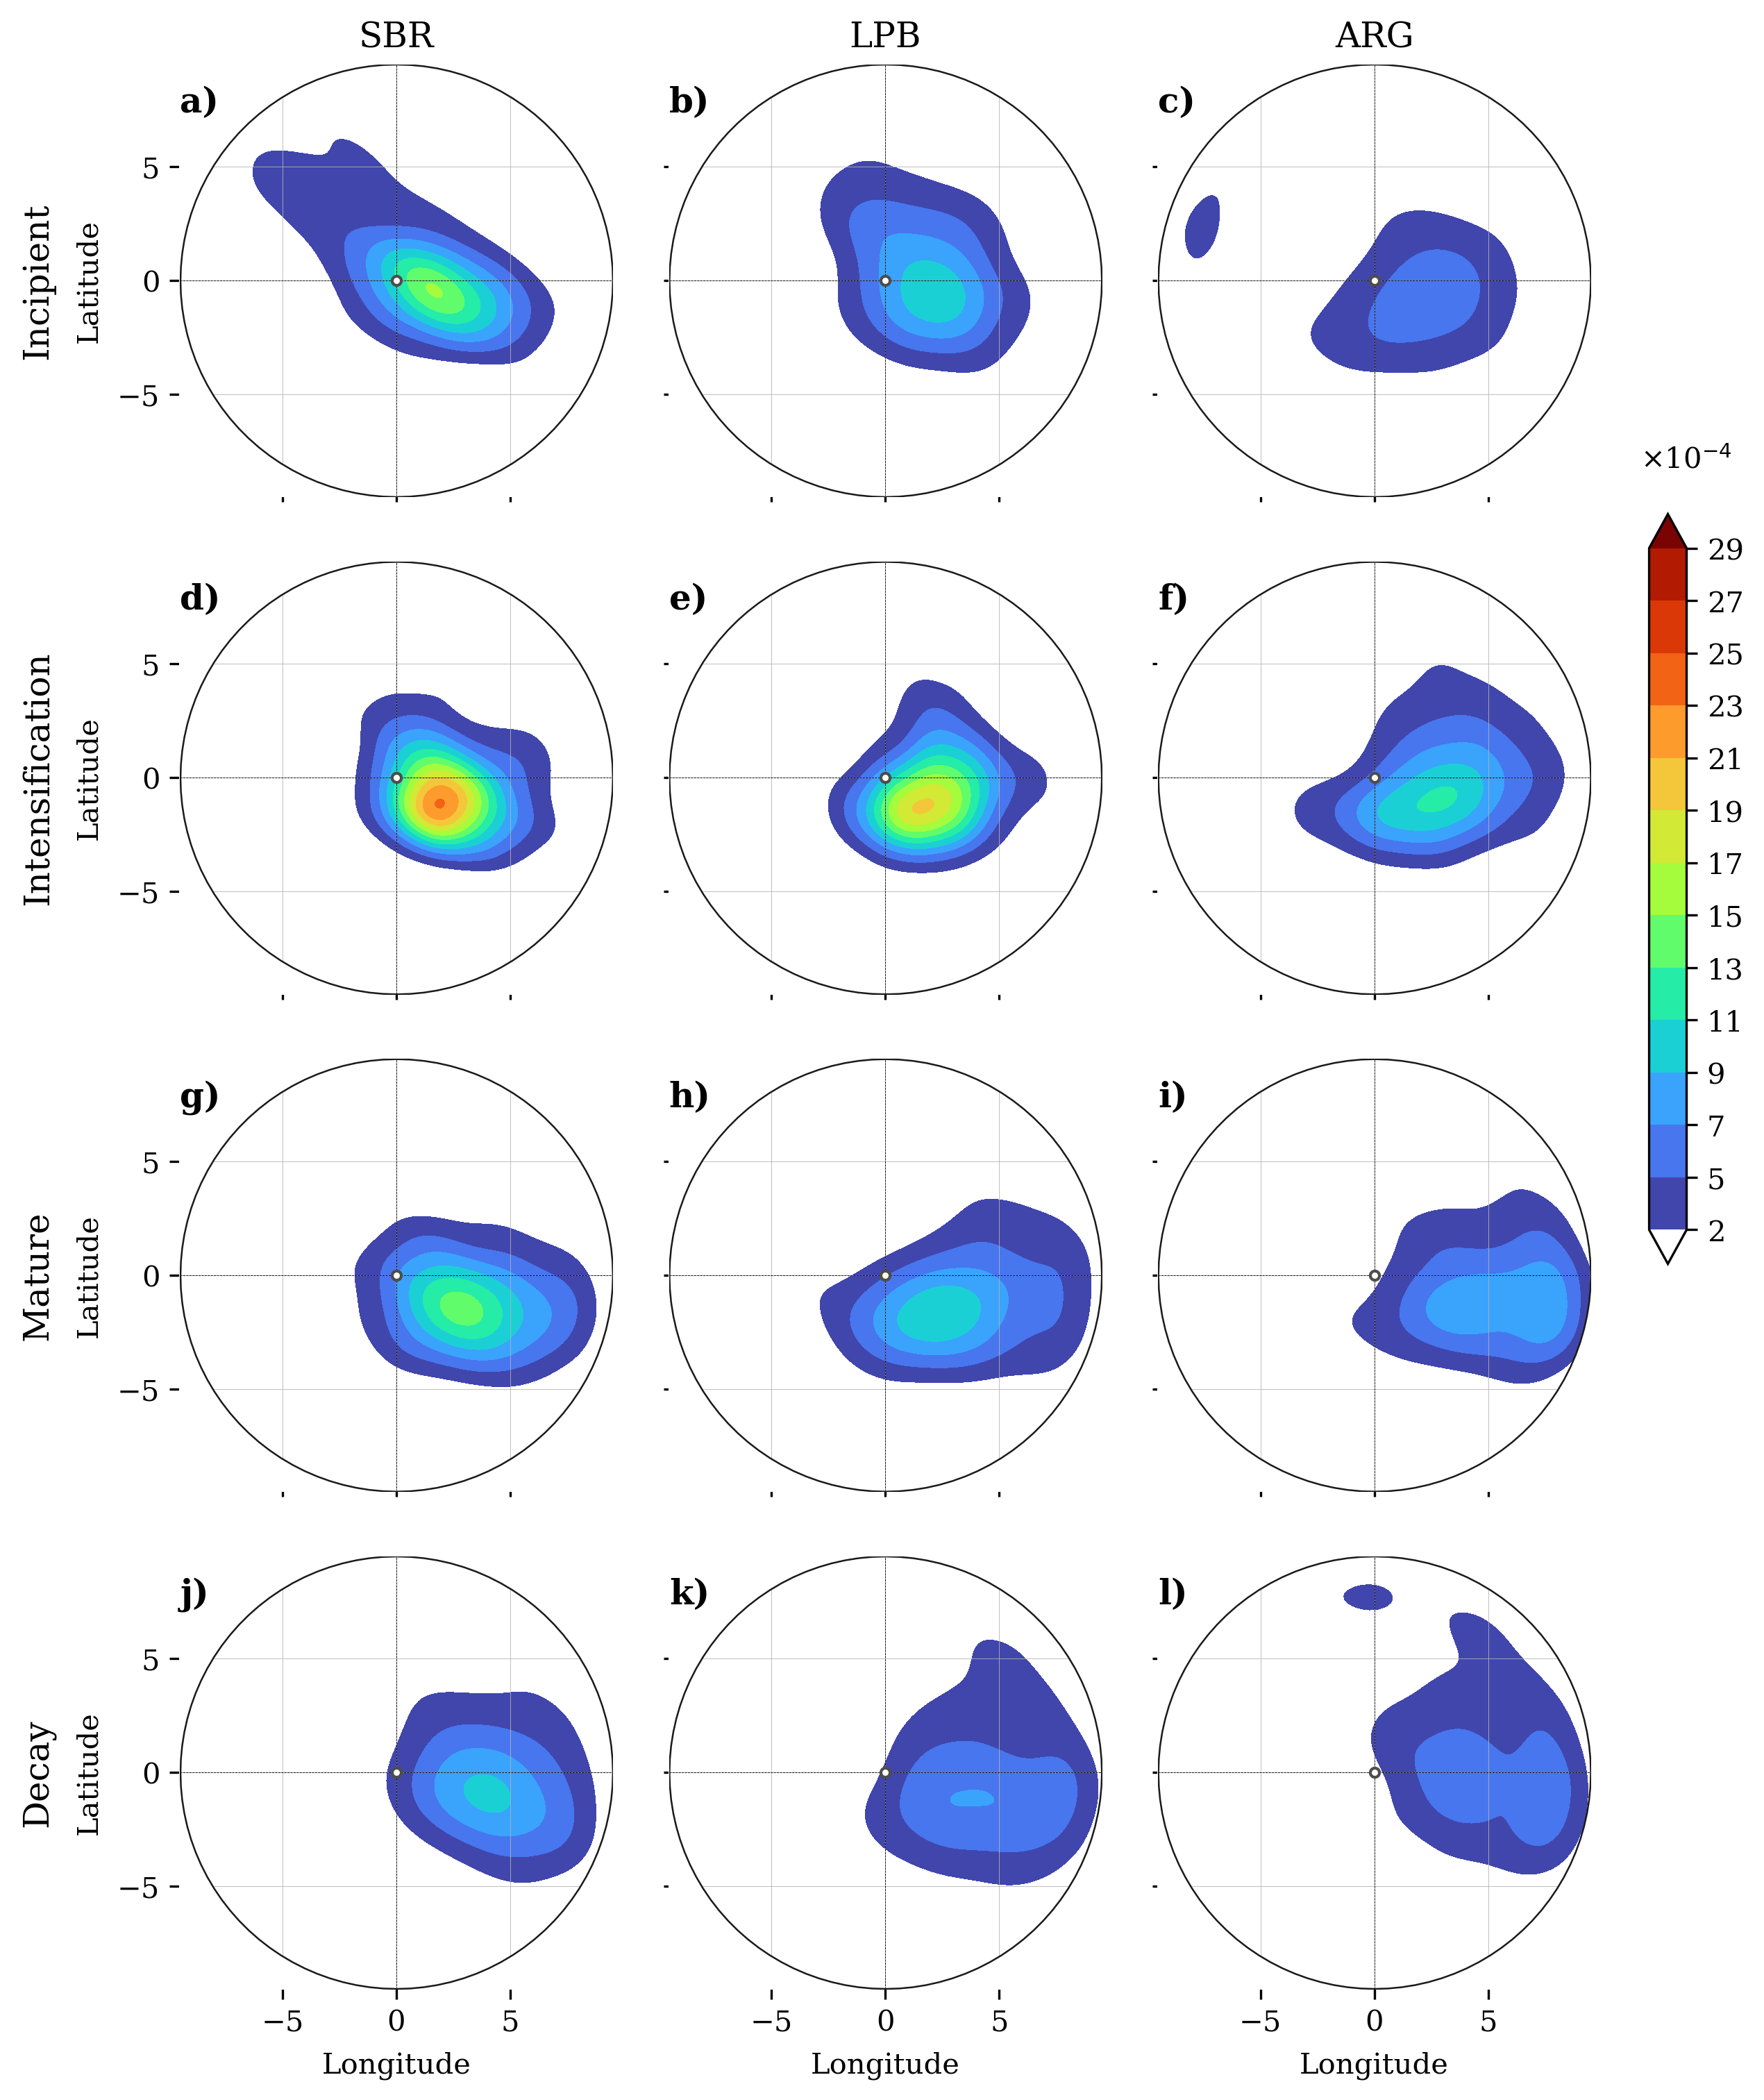
\includegraphics[width=\textwidth]{images/tp/kde_tp_global_fasesxreg.png}
\caption[PDFe de precipitación máxima - Población Global]{Estimación de densidad espacial bidimensional (usando estimación de densidad por kernel KDE) para la ubicación geométrica de los máximos de precipitación total (mm/h) en la Población Global de referencia. La matriz organiza la evolución espacial a través de las fases evolutivas Incipiente (a-c), Intensificación (d-f), Madurez (g-i) y Decaimiento (j-l), segregadas por las regiones de ciclogénesis SBR, LPB y ARG. El dominio lagrangiano abarca $20^{\circ} \times 20^{\circ}$ con centro en el vórtice $(0,0)$. La barra de colores cuantifica la densidad de probabilidad relativa escalada por $10^{-4}$.}
\label{fig:kde_tp_global}
\end{figure}

La Figura~\ref{fig:kde_tp_global} presenta el campo probabilístico derivado con KDE, que mapea la ubicación espacial preferencial de los núcleos de precipitación máxima para la Población Global en el marco lagrangiano.
A diferencia del viento, cuya distribución incipiente ya mostraba difusión centrada en el núcleo, la lluvia máxima presenta desde las etapas iniciales una arquitectura asimétrica respecto al centro del ciclón.

En SBR (panel a), la densidad máxima ($\sim$17$\times10^{-4}$) se concentra en el cuadrante sureste (longitudes 0--5°, latitudes $-$2 a $-$4°), con cola hacia el noroeste, la asimetría más marcada de la fila incipiente. LPB (panel b) presenta un núcleo más compacto ($\sim$13$\times10^{-4}$), también sureste, con elongación al norte. ARG (panel c) es más compleja. Un núcleo principal sureste ($\sim$9$\times10^{-4}$) coexiste con uno secundario en el noroeste (longitudes $-$6 a $-$4°, latitudes $+$2 a $+$4°). La intensificación concentra los picos absolutos. SBR (panel d) alcanza $\sim$29$\times10^{-4}$, máximo de la matriz, con contornos casi circulares en $\pm$3° de longitud y $-$3 a $+$1° de latitud. LPB (panel e) alcanza $\sim$21$\times10^{-4}$, simétrica y centrada, con leve asimetría este (posible influencia orográfica o advección atlántica). ARG (panel f) tiene la densidad más baja ($\sim$13$\times10^{-4}$), núcleo sureste y cola norte ausente en SBR/LPB; la desaparición del núcleo secundario sugiere consolidación hacia un único centro activo.

La mayor densidad de SBR y LPB frente a ARG durante la intensificación se explica no solo por la proximidad a la humedad tropical, sino por los intensos flujos de calor latente y sensible desde el océano que sostienen la convección cerca del frente retrocedido \citep{gozzo2013air}; la advección de aire frío y seco sobre aguas cálidas potencia la evaporación, cuya condensación libera calor que intensifica la circulación y organiza el ascenso en las áreas de mayor precipitación \citep{andrade2024composite}. ARG, sin este forzante oceánico, muestra las densidades más bajas y los patrones más difusos de los paneles c, f, i y l.

Al alcanzar la madurez, las densidades descienden y los patrones se ensanchan. SBR (panel g) cae a $\sim$15$\times10^{-4}$, con el núcleo desplazado al sureste en forma ovalada de eje noroeste-sureste. LPB (panel h) registra el mayor desplazamiento hacia el este de la fila ($\sim$11$\times10^{-4}$). El núcleo migra al sureste y los contornos se elongan hasta $+$6°. ARG (panel i) mantiene asimetría este comparable a LPB pero con densidades más bajas ($\sim$9$\times10^{-4}$), con elongación al noreste que sugiere influencia del flujo zonal.

En el decaimiento, la precipitación se vuelve espacialmente difusa y débil. SBR (panel j) registra su densidad más baja ($\sim$11$\times10^{-4}$), con contornos casi circulares que cubren casi todo el dominio. LPB (panel k) mantiene asimetría este ($\sim$9$\times10^{-4}$), con el núcleo al sureste y el cuadrante oeste prácticamente inactivo. ARG (panel l) revela un núcleo principal sureste ($\sim$7$\times10^{-4}$, la densidad más baja de la figura) que coexiste con uno secundario aislado en el extremo norte, indicando disipación fragmentada en centros débiles.

La asimetría hacia el sector oriental y sureste observada consistentemente en el PDFe de la Población Global (paneles a--f) emerge primariamente de la arquitectura dinámica del WCB. Según el modelo conceptual de \citet{browning1986conceptual} y las evaluaciones observacionales de \citet{naud2020evaluation}, el ascenso inclinado del WCB por delante del frente frío y por encima del frente cálido organiza la precipitación en el flanco cálido del ciclón, patrón documentado de forma consistente en climatologías de ciclones oceánicos de latitudes medias. Este forzante sinóptico constituye el esqueleto dinámico universal de la distribución espacial y explica la carga positiva consistente del EOF1 en el cuadrante sureste (Fig.~\ref{fig:eof1_tp_global}).
A escala global, \citet{catto2015fronts} demuestran una vinculación inequívoca entre los WCB, los frentes activos y la ocurrencia de los eventos de precipitación más intensos en latitudes medias.

Sobre este esqueleto dinámico operan secundariamente moduladores que explican las diferencias entre regiones. En SBR y LPB, la circulación ciclónica induce anomalías positivas de convergencia de humedad acopladas con advección cálida en niveles bajos \citep{cardoso2022synoptic}, organizando la precipitación en bandas noroeste-sureste; el flujo canalizado desde latitudes tropicales hacia el flanco este del vórtice, que \citet{vera2002cold} documenta, intensifica esta asimetría, resultando en núcleos más densos y extendidos (paneles a, b, d, e).
En ARG, la mayor distancia a la humedad tropical y la barrera orográfica de los Andes, ya señaladas en la Sección~\ref{sec:pdf_tp}, atenúan el flujo cálido, generando un patrón más difuso, menos intenso y con estructuras bimodales en las fases inicial y final.

A medida que los sistemas transitan hacia la madurez y decaimiento (paneles g--l), esta firma oriental se expande y difumina, sin foco de convergencia único en los ciclones ordinarios. Esta dispersión refleja la variabilidad estructural de la Población Global; caracterizarla es una necesidad metodológica que permite establecer cómo el ciclón promedio concentra la precipitación en su sector oriental. La separación del subconjunto p90, abordada a continuación, revela estructuras distintas respecto a esta Población Global.

La robustez de este patrón responde en parte a la alta frecuencia de ciclogénesis en las inmediaciones del norte de Argentina, Uruguay y sur de Brasil (${\sim}$18 eventos por invierno), junto con el desplazamiento preferencial de estos sistemas hacia el sureste sobre el océano \citep{mendes2010climatology, simmonds2000mean}, lo que asegura una muestra donde el WCB interactúa sistemáticamente con la configuración regional, sin que esto implique que el contexto climatológico actúe como forzante físico directo en cada evento, sino que funciona como condicionante estadístico que garantiza la representatividad del patrón WCB. Esto justifica el filtrado p90. Si la asimetría oriental es un sustrato climatológico, las diferencias de los ciclones intensos respecto a esa línea base pueden atribuirse con mayor confianza a procesos dinámicos de oclusión, documentada de forma extendida en la cuenca del Atlántico Sur \citep{gramcianinov2019properties}, y no a variabilidad muestral.

\subsection{Subconjunto extremo (p90)}\label{subsec:kde_tp_p90}

\begin{figure}[htbp]
\centering
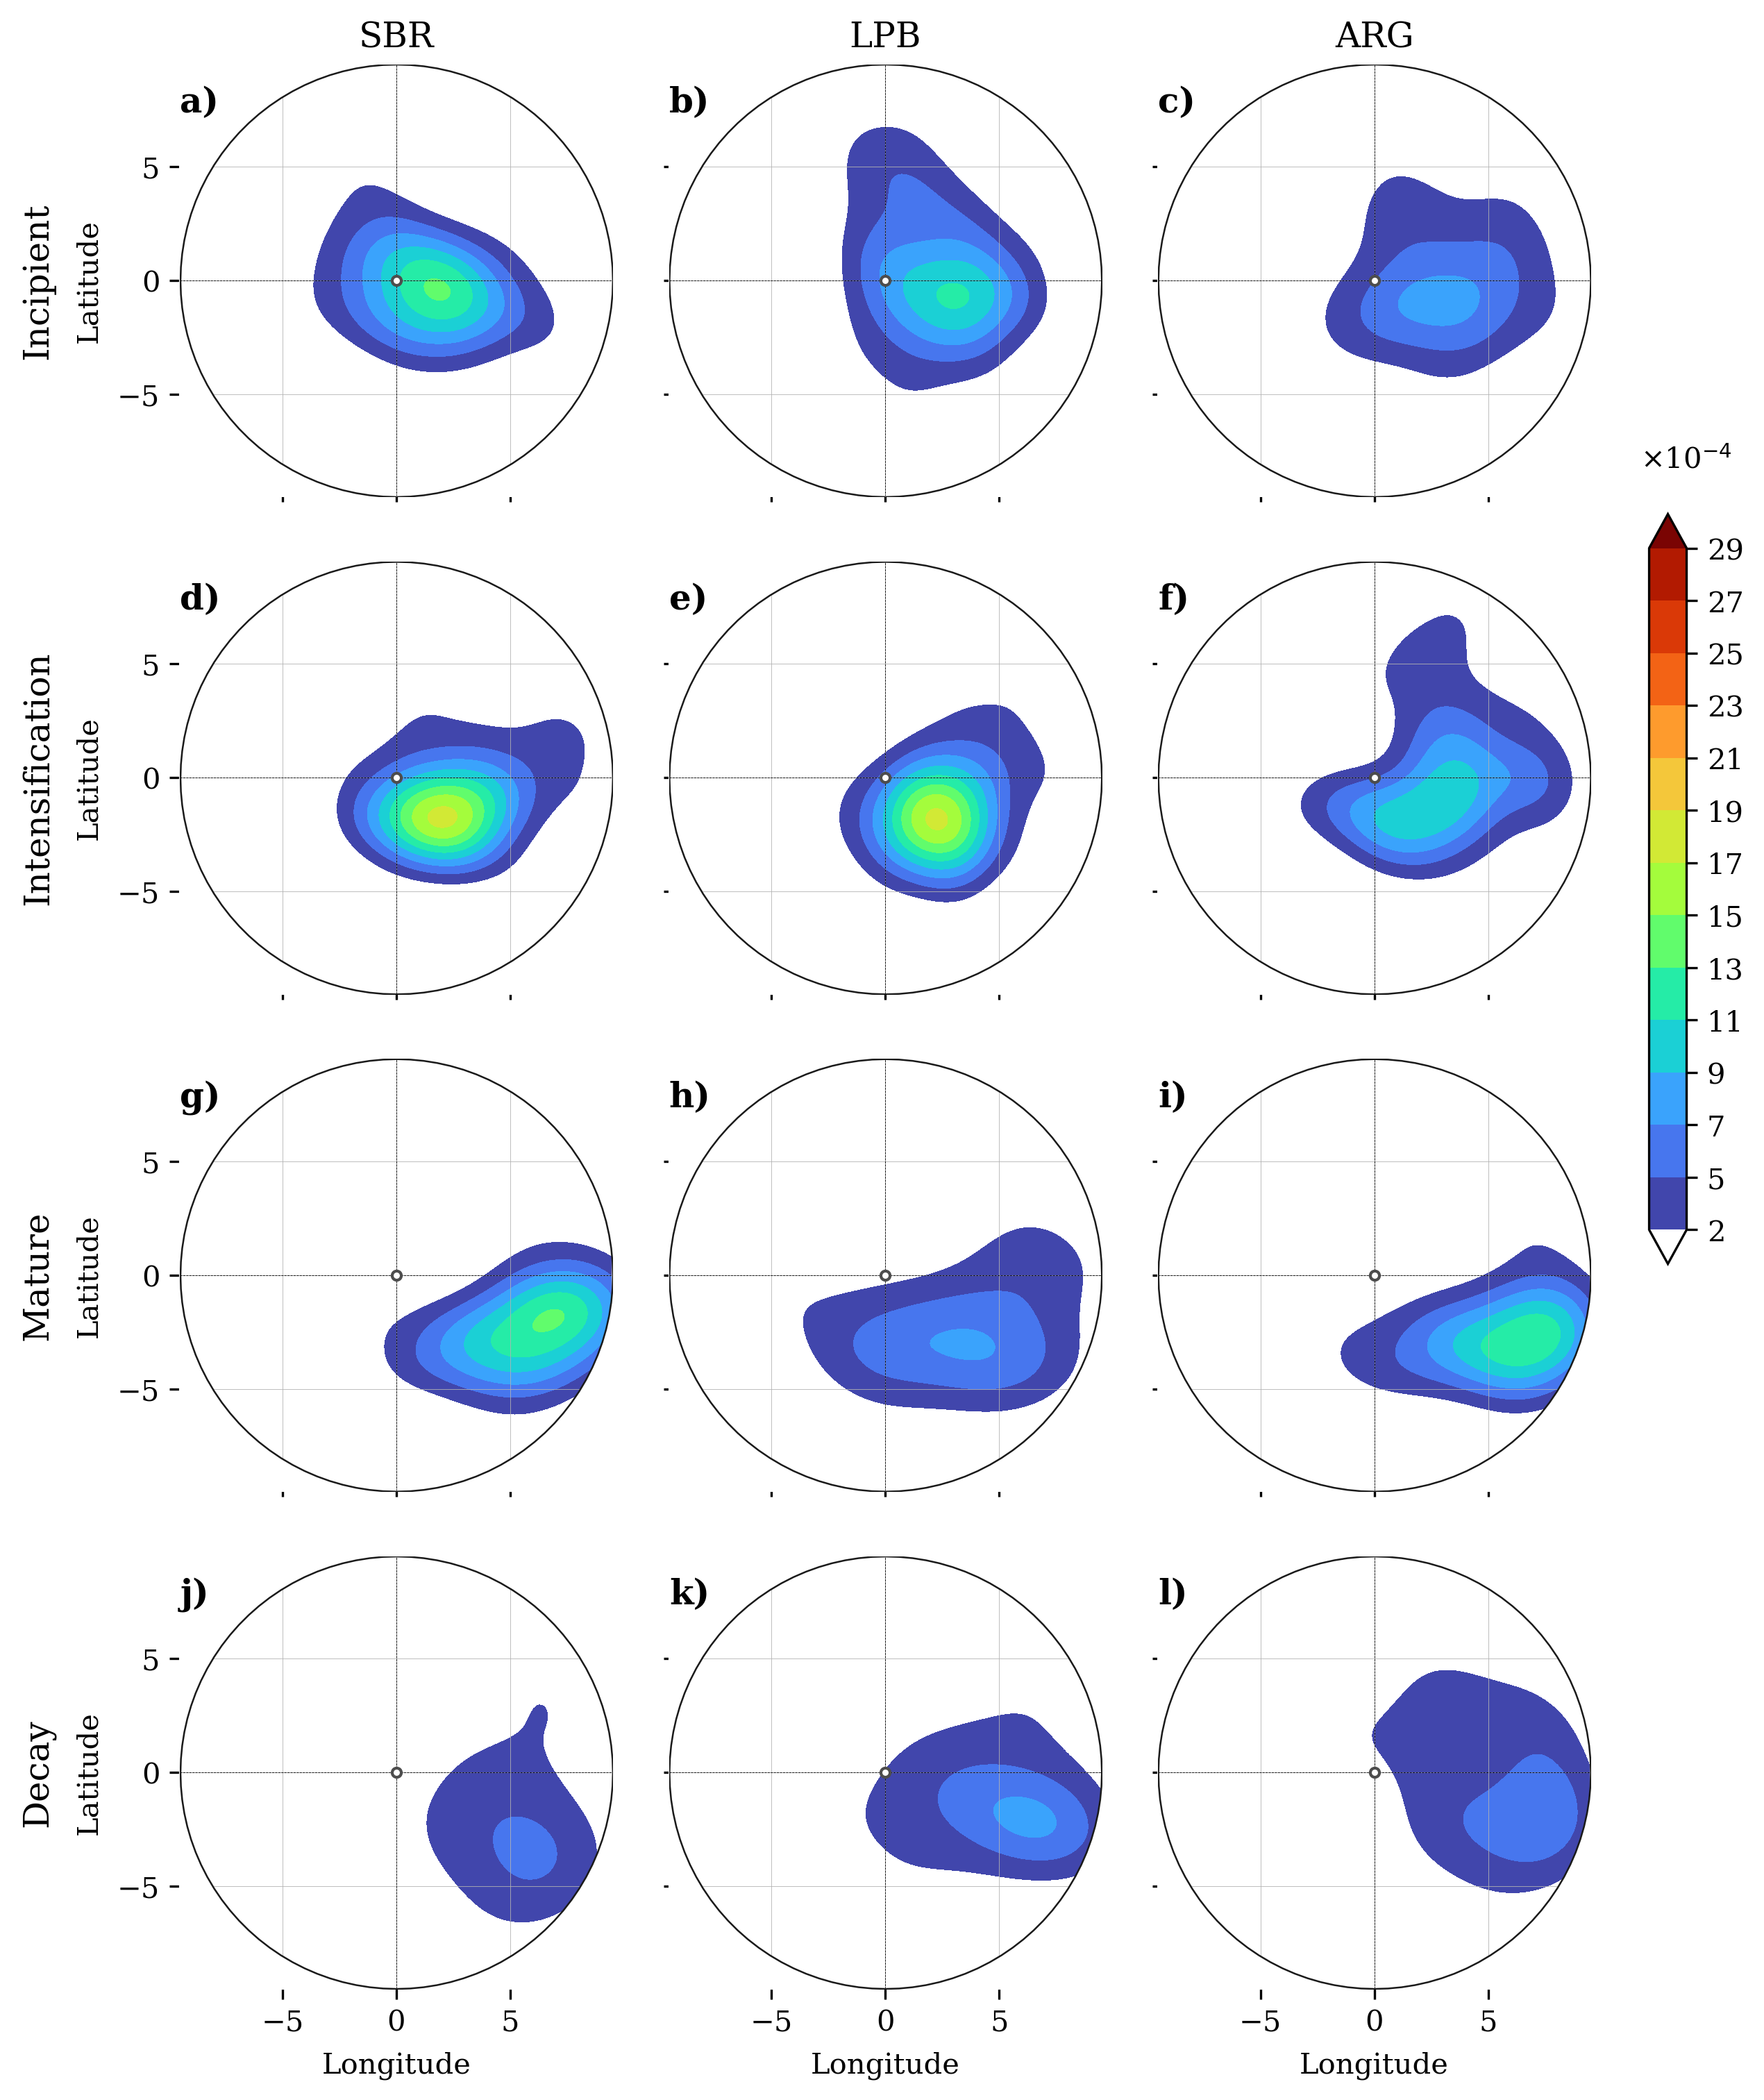
\includegraphics[width=\textwidth]{images/tp/kde_tp_p90_fasesxreg.png}
\caption[PDFe de precipitación máxima - Subconjunto p90]{Estimación de densidad espacial bidimensional (PDFe) para la ubicación geométrica de los máximos de precipitación total (mm/h) correspondiente al subconjunto de ciclones intensos (percentil 90). El formato de los paneles (a-l), la evolución temporal, la segregación regional y la escala colorimétrica ($10^{-4}$) replican la estructura de la Figura~\ref{fig:kde_tp_global}, permitiendo cuantificar el contraste con la Población Global.}
\label{fig:kde_tp_p90}
\end{figure}

Al contrastar la distribución de la Población Global con el estrato p90, la reorganización espacial resulta tan drástica como la observada en el campo de viento, aunque en sentido morfológicamente inverso. La Figura~\ref{fig:kde_tp_p90} revela que la arquitectura pluviométrica de los ciclones más intensos no amplifica la concentración oriental de la Población Global, sino que experimenta un cambio estructural al transitar hacia la madurez.
Dos rasgos son sistemáticos en el contraste con la Población Global: (i) las distribuciones p90 son más compactas en las fases iniciales, filtrando el ruido espacial de baja intensidad; y (ii) el desplazamiento hacia el flanco sureste se acentúa progresivamente desde la intensificación hacia el decaimiento, en bandas estrechas y arqueadas sin equivalente en la Población Global.

En SBR (panel a), la densidad máxima ($\sim$15$\times10^{-4}$) se sitúa en el cuadrante sureste, más compacta que en la Población Global y sin la cola noroeste. El filtrado p90 elimina la actividad precursora alargada, conservando solo el núcleo extremo del flanco sur. En LPB (panel b), el núcleo ($\sim$13$\times10^{-4}$) se desplaza al cuadrante noreste, orientación única en la fila incipiente, asociada al sector norte del sistema. ARG (panel c) simplifica la estructura de la Población Global. Desaparece el núcleo secundario noroeste, conservándose solo el sureste ($\sim$9$\times10^{-4}$), indicando que los eventos extremos incipientes se asocian exclusivamente al núcleo principal.

La intensificación es la fase más simétrica entre la Población Global y p90. SBR (panel d) alcanza $\sim$19$\times10^{-4}$, con el núcleo casi centrado y contornos compactos; aunque inferior al pico de la Población Global ($\sim$29$\times10^{-4}$), la mayor simetría sugiere que el filtrado extremo reduce la variabilidad espacial. LPB (panel e) alcanza $\sim$19$\times10^{-4}$, el panel más simétrico de su columna. ARG (panel f) presenta la densidad más baja de la fila ($\sim$13$\times10^{-4}$), con el núcleo al sureste y una cola norte única en esta fase, sugiriendo una vía secundaria de organización extrema.

Al alcanzar la madurez se produce la reorganización estructural más drástica de la figura. Las densidades máximas se alejan del centro de vorticidad y se confinan en bandas estrechas y arqueadas, dejando el área central y noroccidental sin máximos de lluvia. SBR (panel g) desciende a $\sim$15$\times10^{-4}$, con el núcleo al sureste y contornos elongados al este; la separación del origen es mayor que en la Población Global, indicando que la precipitación extrema madura ocurre en la periferia activa, no sobre el centro. LPB (panel h) registra la asimetría sureste más marcada de la fila ($\sim$9$\times10^{-4}$), con contornos que alcanzan $+$7° y el cuadrante noroeste inactivo. ARG (panel i) presenta elongación este comparable a LPB pero con densidades más altas ($\sim$13$\times10^{-4}$ frente a $\sim$9$\times10^{-4}$ en LPB); la ausencia de la cola norte de la intensificación indica que la organización se simplifica hacia un único núcleo desplazado.

Según \citet{naud2025lifecycle} para el Hemisferio Norte, los ciclones ocluidos desarrollan una cresta térmica que conecta el centro del sistema con el vértice del sector cálido, donde se maximiza la precipitación mediante un forzante de ascenso propio en la periferia. Al alcanzar su máxima intensidad, los p90 intensifican la intrusión seca descrita en la Sección~\ref{sec:pdf_tp} \citep{shapiro1999bridge}, que erradica la nubosidad profunda del núcleo y abre el \textit{dry slot} característico.

Este proceso, descrito en el marco del modelo de Shapiro-Keyser (Sección~\ref{subsec:tb_modelos}), arrastra el remanente de humedad del WCB hacia la periferia, confinándolo en el frente retrocedido (\textit{bent-back front}) y generando la clásica banda de precipitación enroscada (\textit{wrap-around precipitation}) en el cuadrante ocluido, responsable de la nubosidad característica de los sistemas ocluidos \citep{martin1999forcing}; observaciones satelitales en ciclones invernales de latitudes medias del Pacífico noroccidental confirman que esta interacción entre intrusión seca y WCB genera precipitación organizada en banda durante la oclusión \citep{sawada2021heavy}. Se observa en el PDFe durante madurez y decaimiento, geometría arqueada cuyo origen conceptual como \textit{bent-back front} documenta \citet{schultz2021antecedents}.

La intensidad máxima de las precipitaciones está condicionada por la fuerza del WCB y la convección profunda embebida en él a lo largo del frente frío u ocluido \citep{oertel2021warm, blanchard2021warm}; esta convección desencadena corrientes verticales veloces que incrementan el contenido local de hidrometeoros mediante liberación intensa de calor latente.

En el decaimiento, la precipitación se localiza exclusivamente en el flanco sureste, con densidades similares a la Población Global. En SBR (panel j), el núcleo se desplaza al sureste con mayores concentraciones, indicando que los eventos extremos en disipación se organizan preferentemente en el flanco delantero. LPB (panel k) mantiene elongación sureste, con contornos que alcanzan $+$7°. ARG (panel l) presenta asimismo $\sim$7$\times10^{-4}$, con contornos difusos sobre todo el semicírculo este y sin núcleo definido, a diferencia de la Población Global, donde los máximos tienen densidad por debajo del límite al norte del centro.

En eventos sobre regiones de alta disponibilidad de humedad superficial como SBR y LPB, las circulaciones ascendentes convectivas y baroclínicas generan condensación rápida, lo que justifica las densidades agudas y localizadas que distinguen a p90 de la Población Global.
Esta configuración anticipa un desacople de cuadrantes entre los forzantes de viento y precipitación en los ciclones intensos maduros, cuantificado más adelante mediante el EOF1 (Sección~\ref{subsec:eof1_tp_p90}).
% --- SECCIÓN: PATRONES DOMINANTES DE VARIABILIDAD (EOF) - PRECIPITACIÓN ---
\section{Organización estructural: Análisis EOF}\label{sec:eof_tp}

\subsection{Fraccionamiento de varianza}\label{subsec:var_exp_tp}

\begin{figure}[htbp]
\centering
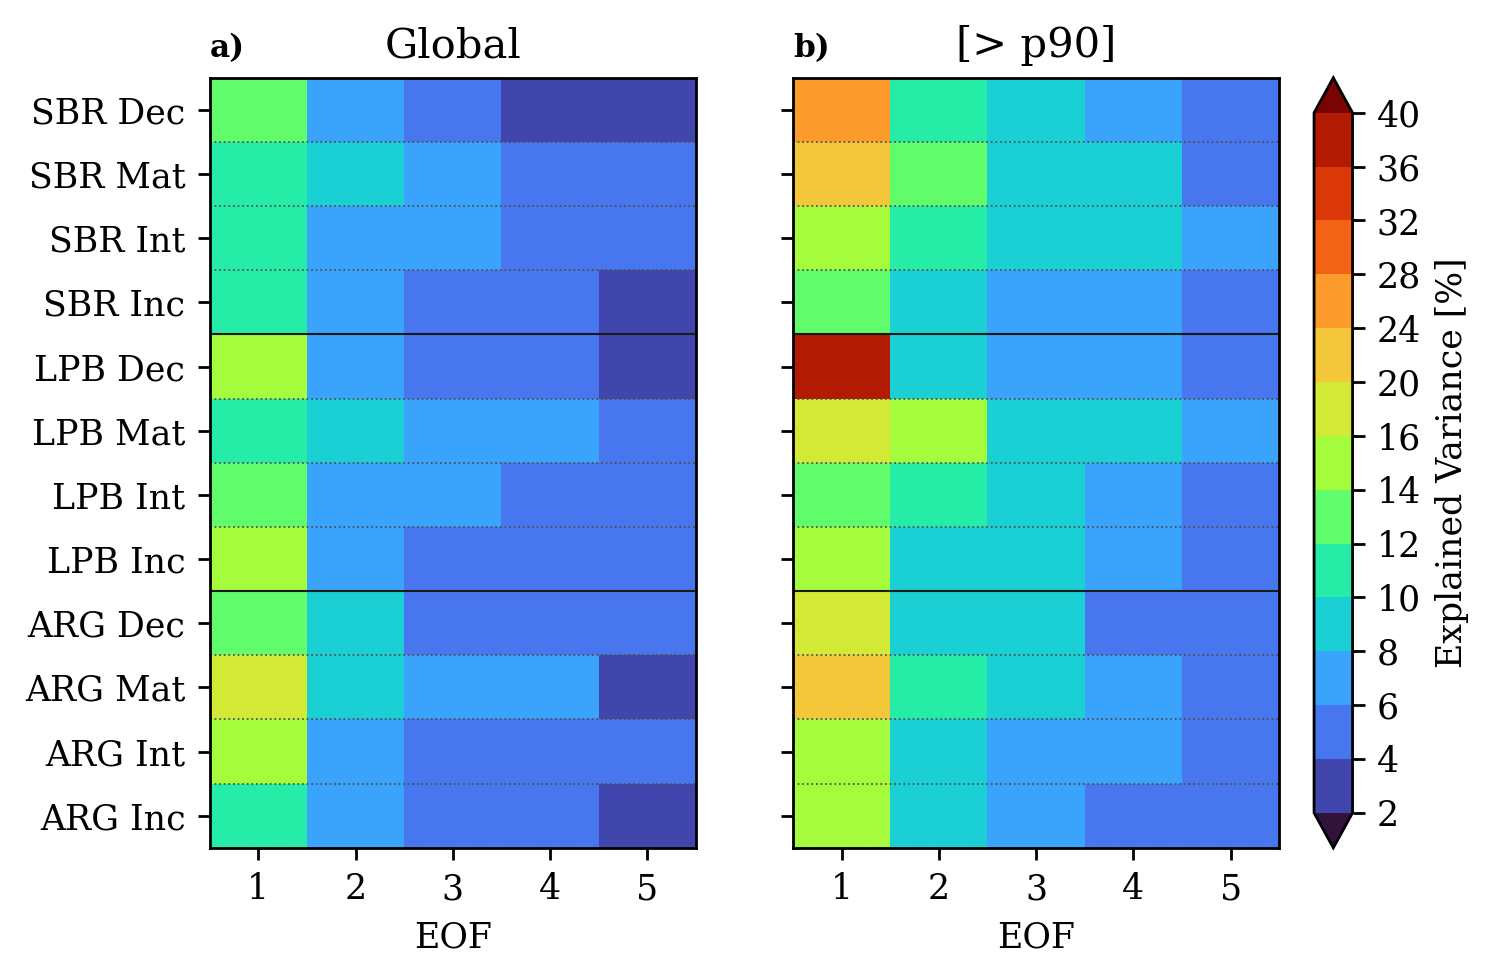
\includegraphics[width=0.8\textwidth]{images/tp/all_expvar_tp_mean2times.png}
\caption[Varianza explicada por los primeros cinco modos (EOF1-EOF5) de precipitación]{Fraccionamiento de la varianza espacial total contenida en los primeros cinco modos dominantes (EOF1 a EOF5) del campo de precipitación total. Se contrasta la distribución de la varianza de la Población Global frente al subconjunto de intensidad (p90) a lo largo del ciclo de vida para cada región de ciclogénesis.}
\label{fig:var_exp_tp}
\end{figure}

La Figura~\ref{fig:var_exp_tp} presenta la distribución porcentual de la varianza espacial explicada por los cinco primeros modos empíricos (PC1 a PC5). Las columnas contrastan la Población Global (panel a) y el subconjunto de intensidad extrema (p90, panel b); las filas corresponden a las doce combinaciones de región de ciclogénesis y fase evolutiva. La escala cromática cuantifica el porcentaje de varianza explicada. Los tonos fríos indican modos dispersos; los cálidos, alta concentración en el modo principal.

En la Población Global (panel a), el espectro de varianza presenta tonos fríos entre los cinco modos en todas las regiones y fases. El EOF1 explica entre 11.1\% y 16.4\% de la varianza total. En SBR oscila entre 11.3\% (madurez) y 13.8\% (decaimiento), sin fase dominante. LPB presenta su máximo en incipiente (14.4\%) y decaimiento (14.3\%), con la madurez como mínimo (11.8\%). ARG exhibe el comportamiento más distintivo. El EOF1 alcanza su máximo en madurez (16.4\%), superando la intensificación (15.6\%), indicando un modo dominante bien diferenciado respecto a SBR y LPB. Los tres primeros modos explican en conjunto aproximadamente 26.8\% (SBR), 28.2\% (LPB) y 31.6\% (ARG) de la varianza total, confirmando que la mayor parte de la variabilidad pluviométrica no queda capturada por unos pocos modos ortogonales.

Este aplanamiento responde a la naturaleza discontinua de la precipitación. A diferencia de las variables de masa, que obedecen a gradientes continuos de gran escala, está gobernada por la actividad frontal, los núcleos de convección embebida y las tasas asimétricas de liberación de calor latente \citep{oertel2021warm}. Según los criterios de \citet{hannachi2007empirical} (Sección~\ref{subsubsec:tb_eof}), esta distribución entre múltiples modos indica que el campo pluviométrico es heterogéneo y requiere varios modos ortogonales para reconstruir la variabilidad observada. \citet{graf2017objective} muestran que la ciclogénesis no opera en categorías discretas sino en un continuo físico donde procesos húmedos y vorticidad potencial son dimensiones cuasi-independientes, explicando la dispersión de energía entre EOFs en las fases iniciales.

En contraste, el subconjunto p90 concentra la varianza explicada por el EOF1 en las fases tardías, con incrementos sistemáticos respecto a la Población Global que se intensifican hacia el final, patrón opuesto al del viento, cuyas mayores varianzas se localizaban en fases tempranas. En SBR, el EOF1 pasa de 11.3\% (Población Global, madurez) a 21.4\% (p90, madurez) y de 13.8\% a 26.2\% en decaimiento (saltos de 10.1 y 12.4 puntos).

En LPB, el incremento ya es notable en madurez (11.8\% a 16\%, $+$4.2 puntos), pero es mayor en decaimiento (14.3\% a 36.5\%, $+$22.2 puntos). ARG muestra los incrementos más moderados ($+$4.3 puntos en madurez, $+$6.8 en decaimiento), coherente con el carácter más gradual de sus oclusiones. En conjunto, los tres primeros modos p90 explican aproximadamente 43.7\% (SBR), 40.8\% (LPB) y 40.4\% (ARG) de la varianza en madurez, frente al 26.8\%, 28.2\% y 31.6\% de la Población Global, confirmando que el filtrado del 10\% más intenso aumenta la organización espacial de la variabilidad.

El comportamiento distintivo de p90 durante el decaimiento, donde el EOF1 concentra hasta 36.5\% de la varianza en LPB, obedece a la consolidación de la banda enroscada como estructura dominante, generando una reducción dimensional efectiva donde el primer modo retiene la mayor fracción posible de la varianza total del campo.

Las diferencias regionales reflejan además la asimetría zonal del tren de ondas baroclínicas del Hemisferio Sur, forzada por la cordillera de los Andes y los contrastes térmicos mar-tierra \citep{inatsu2004zonal}, que fija zonas preferenciales de ciclogénesis y frontogénesis. Esto explica que ARG presente mayor varianza explicada por el EOF1 en las fases iniciales que SBR, donde la convección oceánica introduce mayor variabilidad estructural. Sin embargo, los mayores incrementos de p90 respecto a la Población Global ocurren en SBR y LPB durante las fases no iniciales, donde la humedad oceánica permite que la banda enroscada alcance su mayor coherencia espacial.

Esto revela que la respuesta de la precipitación en la Población Global es difusa, justificando la necesidad de retener múltiples modos; pero prueba también que los p90 poseen la capacidad singular de organizar las precipitaciones en geometrías coherentes, fenómeno sin equivalente en los campos de viento y firma distintiva de los sistemas del Atlántico Sur.


%%%%%%%
\subsection{EOF1 --- Población Global}\label{subsec:eof1_tp_global}

\begin{figure}[htbp]
\centering
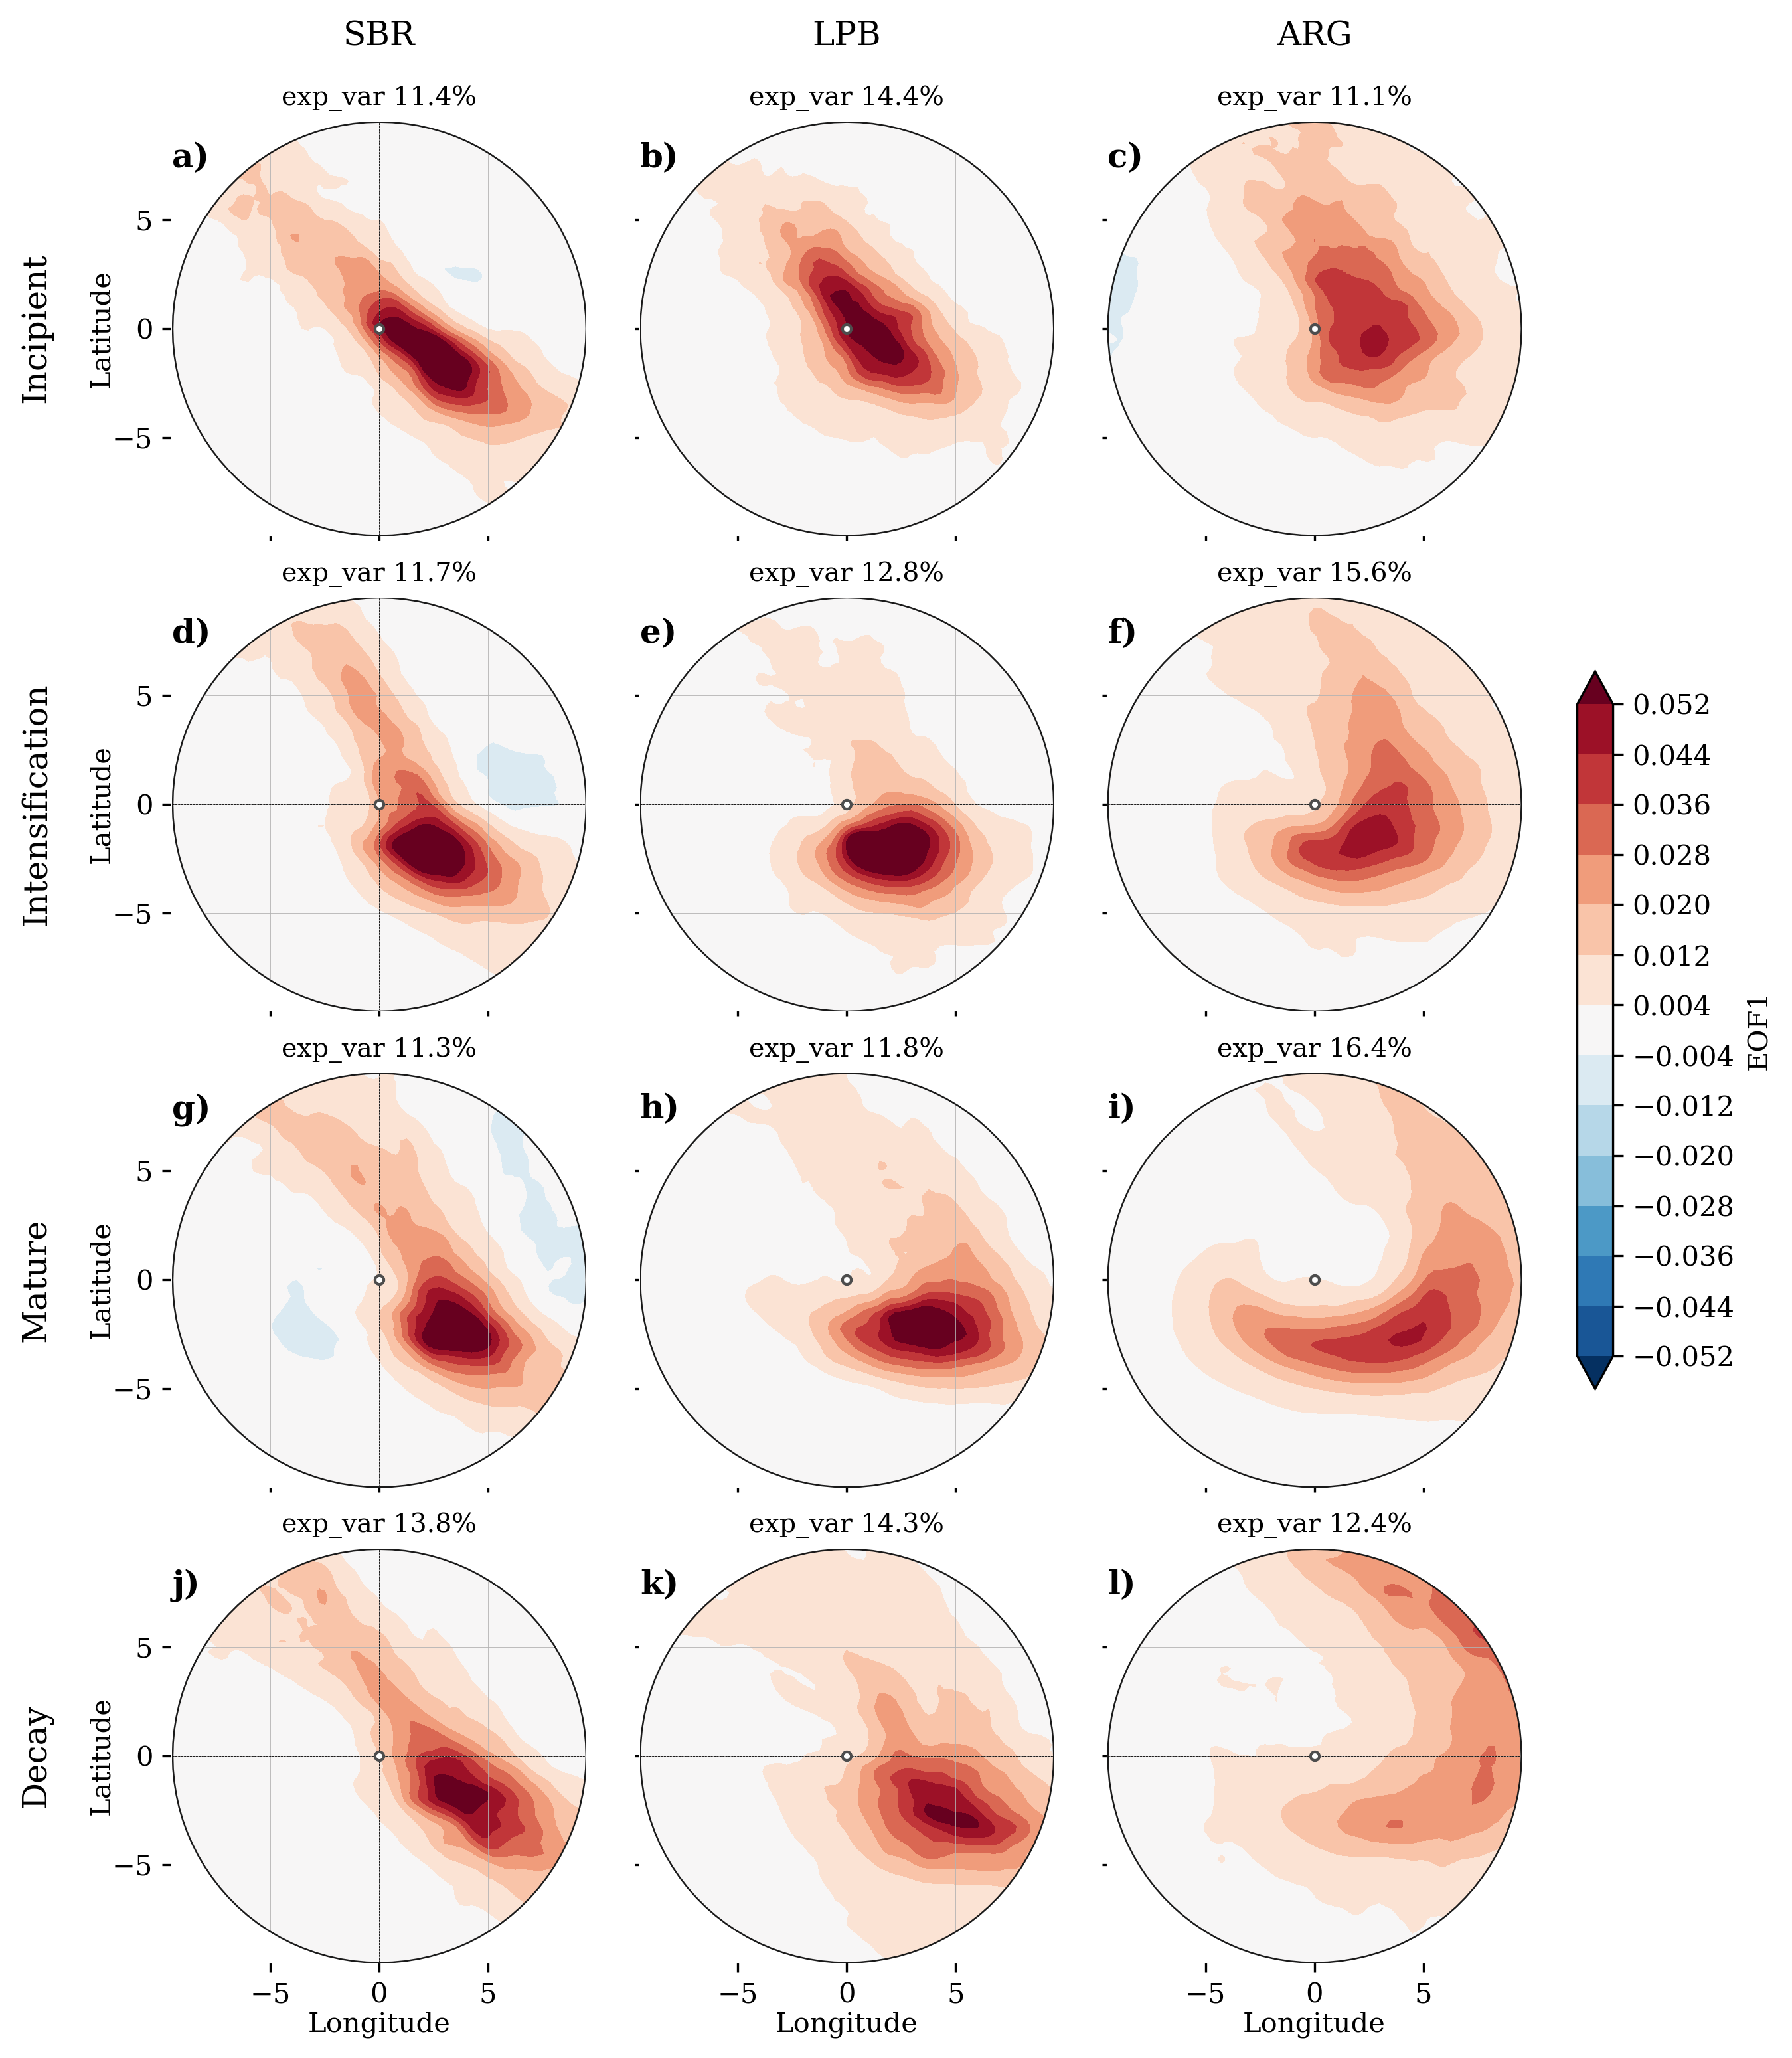
\includegraphics[width=\textwidth]{images/tp/pca1_tp_global_fasesxreg.png}
\caption[EOF1 de precipitación total - Población Global]{Primer modo espacial (EOF1) de la precipitación total (mm/h) para la Población Global de referencia. La disposición matricial organiza la evolución por regiones de ciclogénesis en columnas (SBR, LPB y ARG) y las fases de desarrollo evolutivo en filas (Incipiente, Intensificación, Madurez y Decaimiento). Sobre cada panel se indica el porcentaje de la varianza espacial total explicada (\textit{exp\_var}) por esta componente principal. La escala cromática divergente cuantifica las anomalías estructurales relativas al centro del vórtice.}
\label{fig:eof1_tp_global}
\end{figure}

La Figura~\ref{fig:eof1_tp_global} presenta los patrones espaciales del primer modo empírico (EOF1) de la precipitación total, con la misma disposición matricial de los campos PDFe previos, un dominio circular lagrangiano de 20 grados con contornos que representan anomalías estructurales respecto a la media. Los porcentajes de varianza explicada oscilan entre 11.1\% y 16.4\%, confirmando la baja dominancia del primer modo respecto al viento a 10 metros y la naturaleza discontinua e intermitente del campo pluviométrico.

En SBR, el EOF1 mantiene una estructura consistente a lo largo del ciclo de vida, con un núcleo positivo máximo ($\sim$0.052) anclado al cuadrante sureste y una cola elongada hacia el noroeste, formando una banda diagonal que atraviesa el dominio, la misma orientación del WCB descrita en la Sección~\ref{subsec:kde_tp_global}.

En la fase incipiente (panel a, 11.4\%), el núcleo sureste coexiste con la cola noroeste y pequeñas zonas negativas ($\sim$$-$0.004 a $-$0.012) en el este. En la intensificación (panel d, 11.7\%), los contornos se vuelven más simétricos y aparece mayor área negativa en el noreste, creando un dipolo positivo-negativo. En la madurez (panel g, 11.3\%), el núcleo se aleja del origen hacia el sureste, con valores negativos en oeste y noreste que acentúan el carácter dipolar. El decaimiento (panel j, 13.8\%) muestra aumento de varianza y desaparición de los valores negativos, resultando en un monopolo positivo puro elongado diagonalmente.

LPB presenta los patrones más simétricos y compactos. En la fase incipiente (panel b, 14.4\%), el núcleo positivo máximo ($\sim$0.052) se centraliza en torno al origen, con contornos casi circulares y sin valores negativos; su mayor varianza en esta fase (14.4\% frente a 11.4\% de SBR y 11.1\% de ARG) indica un modo dominante más robusto y reproducible. En la intensificación (panel e, 12.8\%), el núcleo migra al sureste con contornos casi perfectamente simétricos, la simetría más notable de la fase. En la madurez (panel h, 11.8\%), el núcleo se desplaza ligeramente al este con contornos elongados. El decaimiento (panel k, 14.3\%) muestra aumento de varianza, con el núcleo al sureste y una cola positiva hacia el norte.

ARG exhibe el comportamiento más distintivo y asimétrico. En la fase incipiente (panel c, 11.1\%), el núcleo positivo ($\sim$0.052) se ubica en el sureste con elongación al norte y un débil dipolo al oeste; su varianza es la más baja de la figura, reflejando la alta variabilidad no estructurada de la región en esta fase. La intensificación (panel f, 15.6\%) presenta el valor más alto de esta fase en la Población Global, con el núcleo sureste manteniendo su posición desplazada y una cola norte ausente en SBR y LPB. A diferencia de las regiones oceánicas, en ARG el modo dominante permanece sesgado hacia el flanco delantero incluso en intensificación. La madurez (panel i, 16.4\%) alcanza el máximo absoluto de la figura global, único entre las tres regiones, SBR y LPB tienen su pico en decaimiento e incipiente, respectivamente, indicando una organización espacial excepcionalmente reproducible en Argentina. El decaimiento (panel l, 12.4\%) muestra valores positivos difusos sobre el semicírculo este sin núcleo definido, contrastando con los patrones más estructurados de SBR y LPB.

La banda de anomalías positivas orientada noroeste-sureste que muestra el EOF1 es la expresión del WCB (Sección~\ref{subsec:kde_tp_global}). Las diferencias regionales de intensidad reflejan además la disponibilidad de humedad remota que alimenta al WCB. Según \citet{gozzo2017climatology}, la ciclogénesis en el Atlántico Sudoccidental depende principalmente del transporte de vapor desde el Atlántico tropical, con un aporte secundario de los flujos locales de calor latente por evaporación, mientras que \citet{rocha2016estudio} documentan que la convergencia en 850~hPa facilita un aporte constante de humedad desde la Amazonía hacia la zona de formación en SBR, explicando por qué el EOF1 presenta anomalías más intensas y concentradas en SBR y LPB, y un patrón más difuso en ARG.
Esta baja varianza explicada por el primer modo, consistente con la naturaleza discontinua de la precipitación (Sección~\ref{subsec:var_exp_tp}), constituye la línea base dispersa que permite dimensionar la transformación estructural que experimentan los eventos p90 al ocluirse, cuando abandonan este comportamiento transitorio para confinar la precipitación en geometrías estructuradas, como se examina a continuación.

\subsection{EOF1 --- Subconjunto p90}\label{subsec:eof1_tp_p90}

\begin{figure}[htbp]
\centering
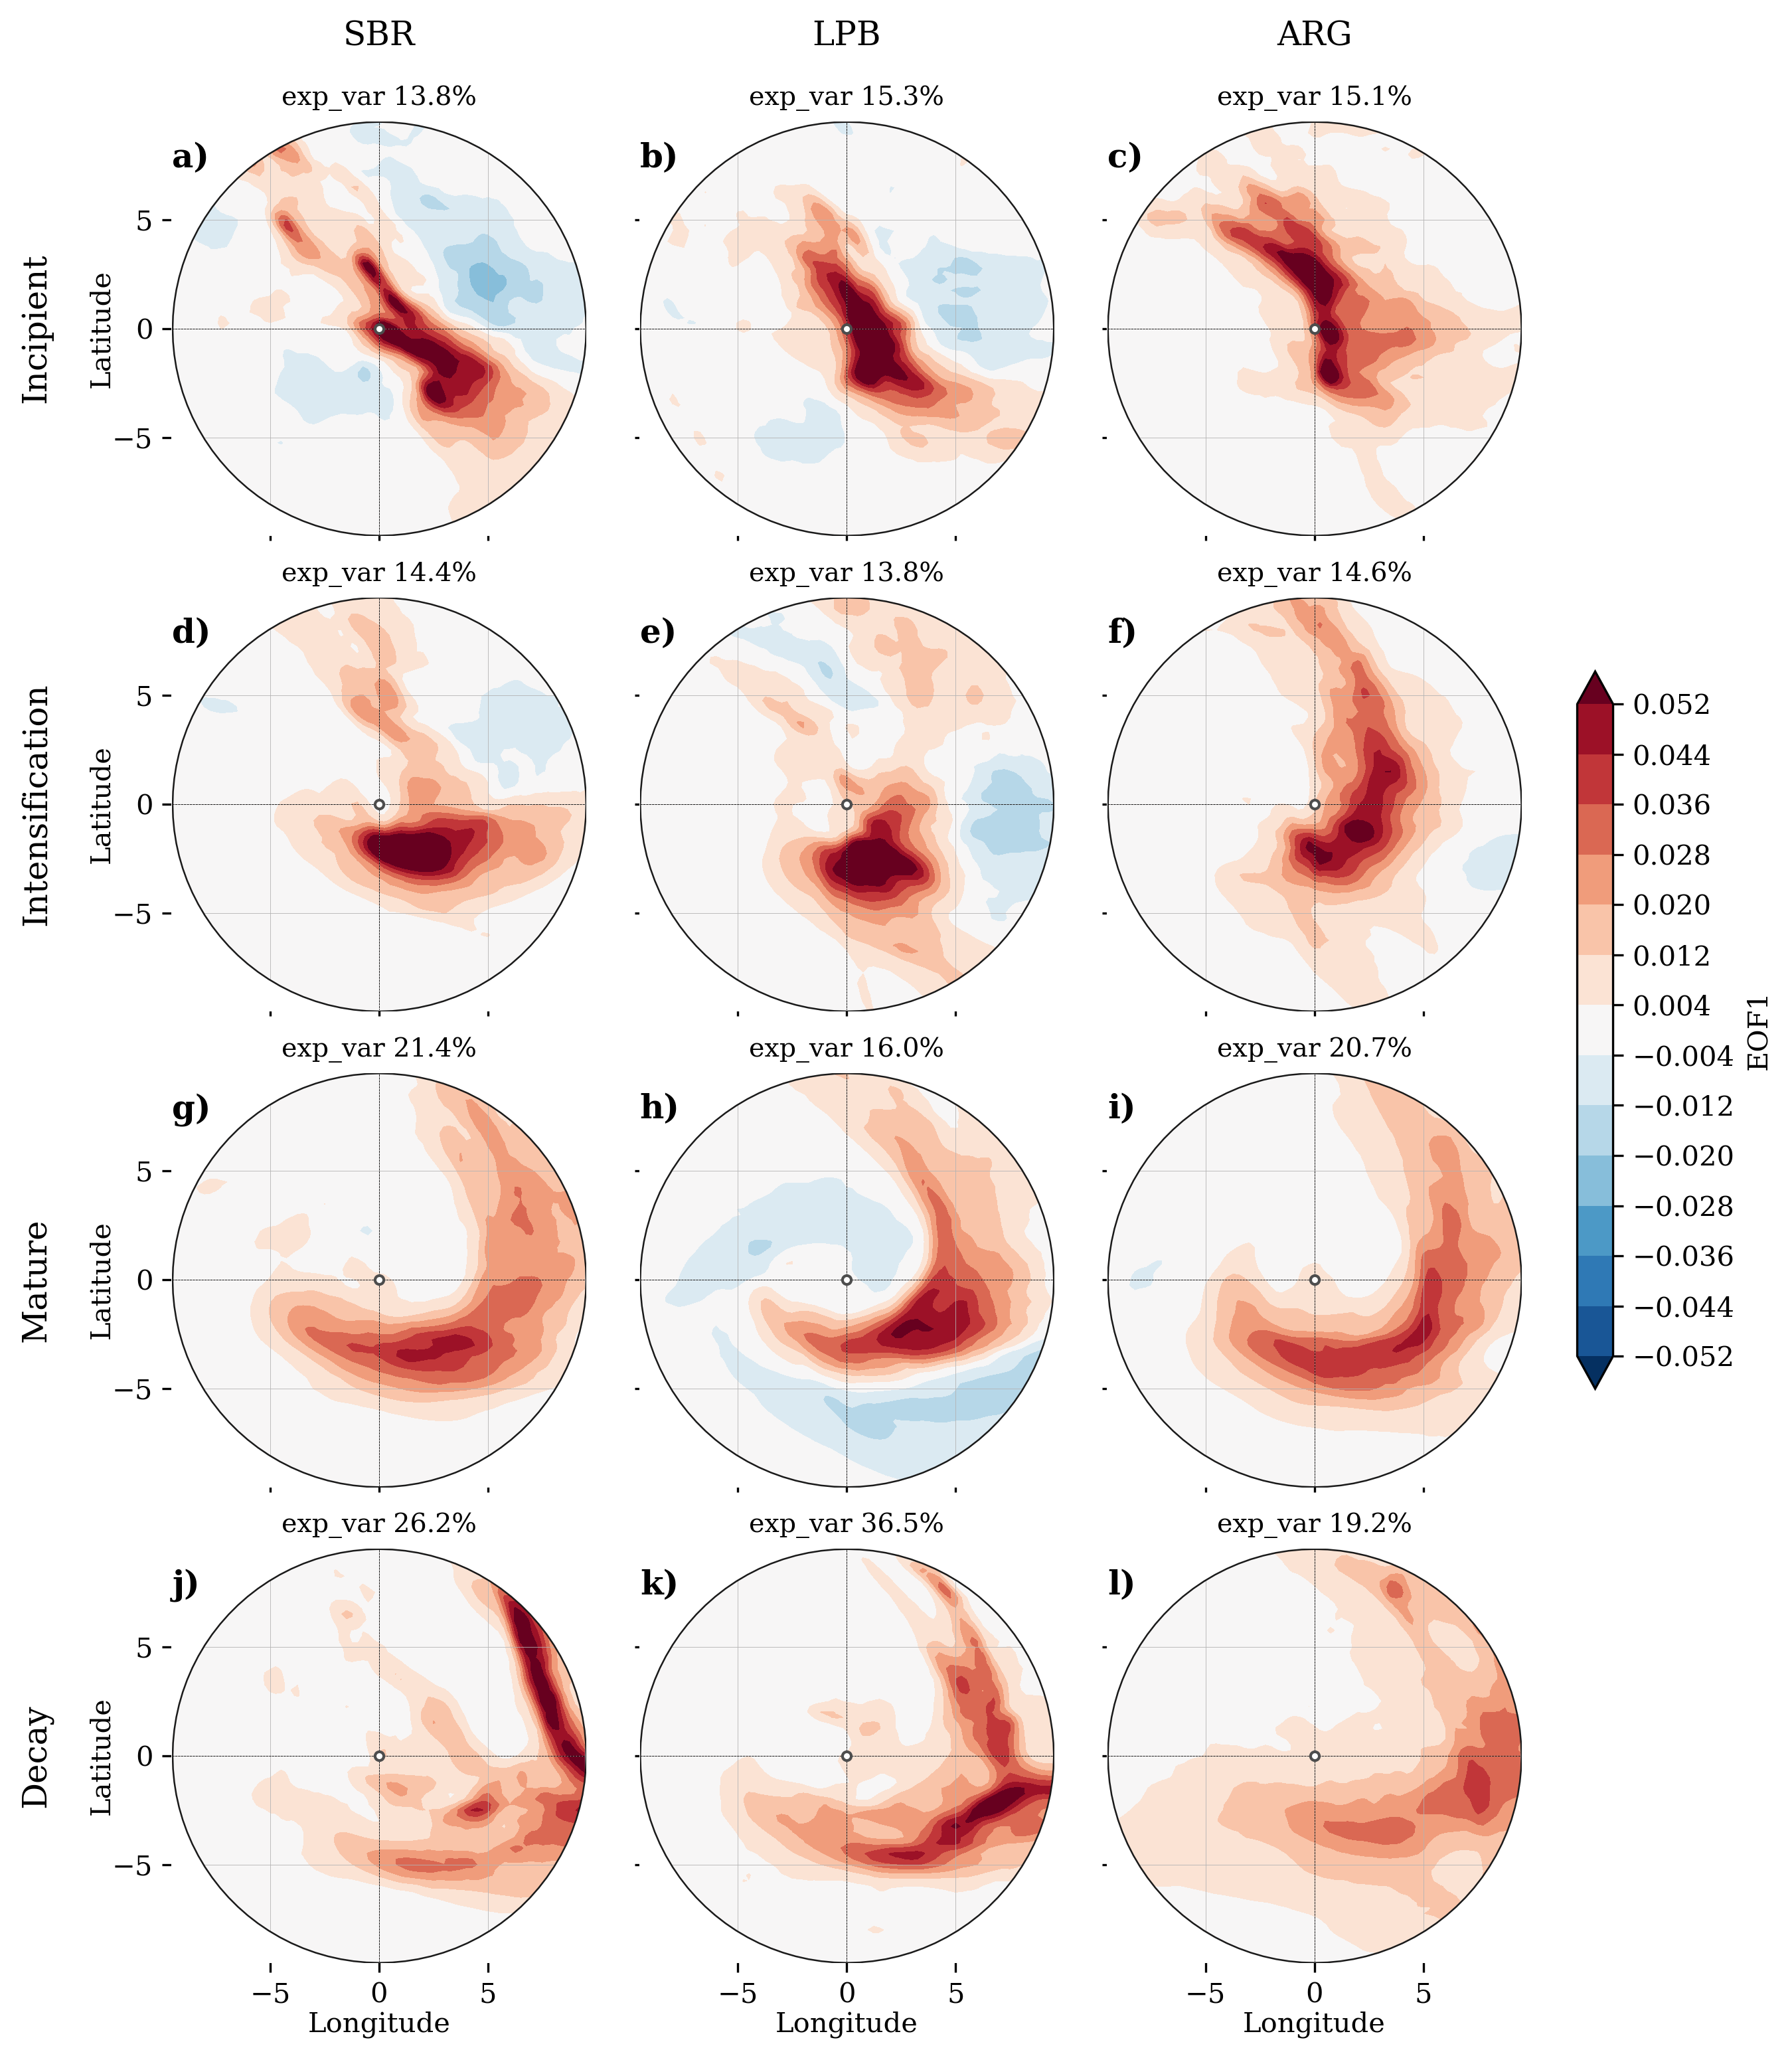
\includegraphics[width=\textwidth]{images/tp/pca1_tp_p90_fasesxreg.png}
\caption[EOF1 de precipitación total - Subconjunto p90]{Primer modo espacial (EOF1) de la precipitación total (mm/h) para el estrato de ciclones intensos (percentil 90). El formato de los paneles (a-l), la nomenclatura de varianza explicada y el dominio espacial mantienen una correspondencia estricta con la Figura~\ref{fig:eof1_tp_global}, permitiendo cuantificar la profunda transformación estructural que experimentan los sistemas severos, especialmente durante su oclusión final.}
\label{fig:eof1_tp_p90}
\end{figure}

La Figura~\ref{fig:eof1_tp_p90} presenta los patrones espaciales del primer modo para el estrato p90, con la misma disposición matricial de la Población Global. El contraste con la Figura~\ref{fig:eof1_tp_global} es inmediato. El filtrado p90 produce dos efectos sistemáticos en todas las regiones y fases: un incremento generalizado de la varianza explicada por el EOF1, más pronunciado en las fases tardías, y una transformación morfológica que convierte los monopolos y dipolos de la población general en estructuras arqueadas durante madurez y decaimiento.

Durante las fases iniciales, el filtrado p90 refina los patrones del global sin transformarlos radicalmente. En SBR, la incipiente (panel a, 13.8\%, $+$2.4 puntos) muestra una banda diagonal noroeste-sureste con zonas negativas ($\sim$$-$0.012 a $-$0.028) en el noreste, conformando un dipolo más nítido; la intensificación (panel d, 14.4\%, $+$2.7 puntos) mantiene el núcleo próximo al origen, más compacto, con la zona negativa mejor delimitada. En LPB, la incipiente (panel b, 15.3\%, $+$0.9 puntos) mantiene la banda diagonal, más estrecha, con zonas negativas similares; la intensificación (panel e, 13.8\%, $+$1.0 puntos) cambia de monopolo compacto a dipolo, con el polo positivo aún al sureste. En ARG, la incipiente (panel c, 15.1\%, $+$4.0 puntos) muestra la simplificación más notable. La banda diagonal es más definida que en el global y desaparece el débil dipolo; la intensificación (panel f, 14.6\%, $-$1.0 puntos) mantiene el núcleo sureste con la cola norte, con valores negativos mínimos ausentes en el global. La intensificación es, en conjunto, la fase más estable entre global y p90, sugiriendo que los mecanismos de organización durante el desarrollo activo no difieren cualitativamente entre sistemas ordinarios y más intensos.

La madurez es donde se produce la transformación morfológica más drástica. En SBR (panel g, 21.4\%, $+$10.1 puntos), el patrón del global es reemplazado por un monopolo positivo en arco desde el suroeste hasta el noreste, con el cuadrante noroccidental libre de anomalías positivas, primera manifestación clara de la banda enroscada como modo dominante. LPB (panel h, 16\%) registra el salto más extraordinario de la figura. El núcleo positivo ($\sim$0.052) forma un arco que envuelve el sistema desde el suroeste hasta el noreste, con zonas negativas ($\sim$$-$0.012 a $-$0.036) en el noroeste que crean el dipolo más marcado de la figura p90. ARG (panel i, 20.7\%, $+$4.3 puntos) presenta un arco similar pero de menor extensión y valores negativos mínimos, resultando en un monopolo arqueado sin dipolaridad.

En el decaimiento, las estructuras se distorsionan y desplazan hacia el flanco oriental externo. En SBR (panel j, 26.2\%, $+$12.4 puntos), el núcleo positivo se concentra en una banda que bordea el extremo este del dominio. LPB (panel k, 36.5\%) muestra un arco en forma de "L" invertida desde el sur hasta el este. ARG (panel l, 19.2\%, $+$6.8 puntos) presenta el patrón más difuso de la fila, similar en morfología al global.

Las estructuras arqueadas que emergen en el EOF1 corroboran que la banda enroscada, ya identificada en la PDFe (Sección~\ref{subsec:kde_tp_p90}), constituye el modo dominante de variabilidad espacial una vez que la intrusión seca desplaza la humedad del núcleo hacia la periferia. El EOF1 la cuantifica como el patrón que explica 21.4\% (SBR) y 20.7\% (ARG) de la varianza total en madurez, y 36.5\% (LPB) en decaimiento, evidenciando que su geometría es estadísticamente replicable y no un artefacto de eventos aislados.

La localización e intensidad de esta banda dependen secundariamente de los flujos de calor latente oceánico ya discutidos (Sección~\ref{subsec:kde_tp_global}). Calientan la baja troposfera y retroalimentan las corrientes verticales, anclando las áreas de máxima varianza y permitiendo que la banda enroscada alcance sus tasas más elevadas sobre SBR y la cuenca atlántica adyacente, donde el contraste térmico oceánico es más pronunciado.

El mantenimiento de esta arquitectura durante el decaimiento responde a procesos de retroalimentación diabática internos. Según \citet{reboita2022from}, el calentamiento diabático reduce el cizallamiento vertical del viento y facilita el alineamiento entre los sistemas de niveles bajos y altos, consolidando la seclusión cálida y desacoplando la dinámica pluviométrica de las fluctuaciones lineales del gradiente sinóptico de fondo, de modo que la banda enroscada persiste mientras el ciclón se disipa.

Según el espacio de fases de \citet{hart2003cyclone}, el paso a la madurez y decaimiento en p90 implica el desarrollo de seclusiones cálidas como régimen evolutivo distintivo; dentro de este marco general, la forma específica de la banda arqueada del EOF1 deriva de los procesos de oclusión y forzantes oceánicos ya descritos.

Al contrastar estos patrones con los campos de viento equivalentes (Sección~\ref{subsec:eof1_wind10_p90}), se evidencia geométricamente el desacople espacial de los forzantes, mientras la variabilidad de las ráfagas más intensas se compacta en el cuadrante noroeste (cinta transportadora fría), la lluvia remanente se organiza en una herradura sólida en los cuadrantes sureste y sur, con los valores negativos confinados al oeste en LPB y al noroeste en SBR, confirmando la separación geométrica entre el forzante eólico y el pluviométrico en los ciclones más intensos del Atlántico Sur.

\subsection{Significancia estadística}\label{subsec:significancia_tp}

Para discriminar entre señales físicas robustas y fluctuaciones propias del remuestreo, se evalúa la significancia estadística de los autovectores espaciales mediante el método Bootstrap-$t$ (Sección~\ref{subsec:bootstrap_significancia}). Este análisis se concentra en la fase de madurez, el momento de mayor señal dinámica y de mayor interés para el argumento central de esta tesis, como verificación representativa de que los patrones EOF documentados en las demás fases no son artefactos del muestreo. La Figura~\ref{fig:xeof_madurez_global_tp} documenta los tres primeros modos (EOF1--EOF3) y sus series temporales (PC1--PC3) para la Población Global en madurez; la Figura~\ref{fig:xeof_madurez_p90_tp} presenta el análisis equivalente para p90. El achurado delimita las áreas con cargas espaciales estadísticamente significativas al 95\%.

\begin{figure}[htbp]
\centering
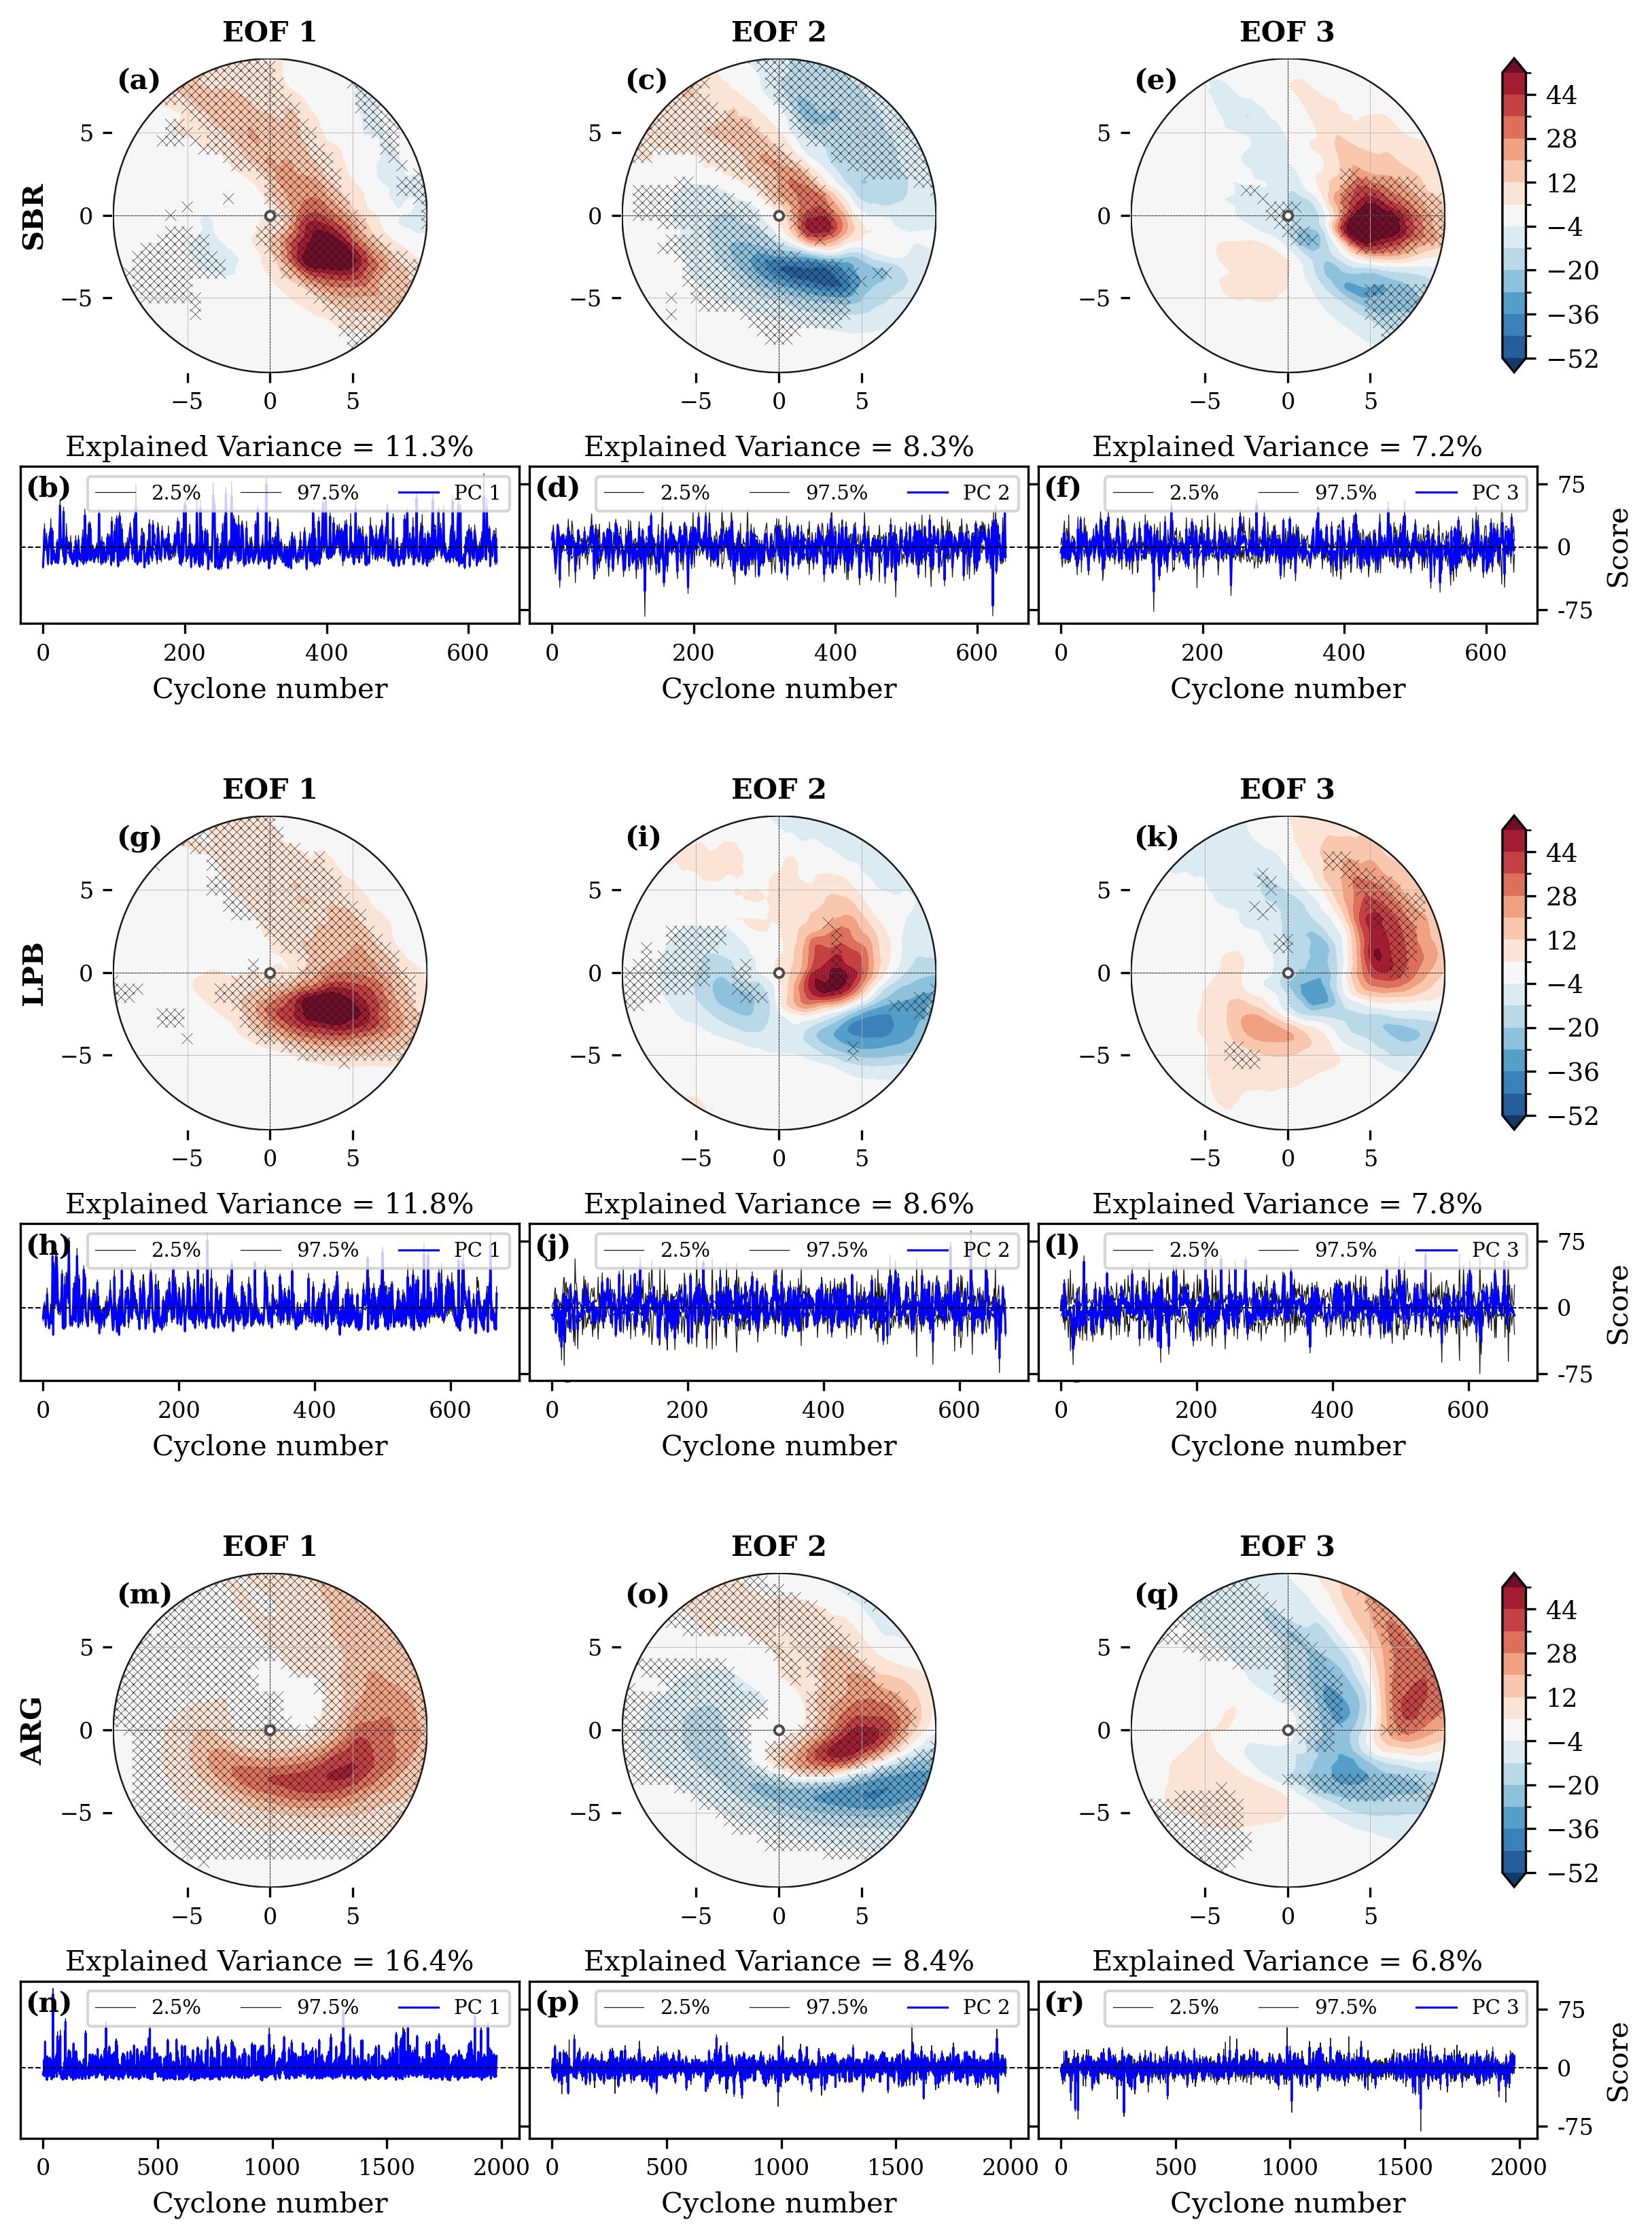
\includegraphics[width=\textwidth]{images/tp/xeof_global_tp_mature.png}
\caption[Significancia espacial de los EOFs en fase de madurez - Población Global (tp)]{Descomposición EOF de la precipitación total para la Población Global en fase de madurez. Paneles (a, c, e): mapas de los tres primeros modos espaciales (EOF1--EOF3) con achurado indicando significancia estadística al 95\% (test Bootstrap-$t$). Paneles (b, d, f): series temporales correspondientes de las Componentes Principales (PC1--PC3). La línea gris delimita los percentiles 2.5 y 97.5 de la distribución bootstrap.}
\label{fig:xeof_madurez_global_tp}
\end{figure}

\begin{figure}[htbp]
\centering
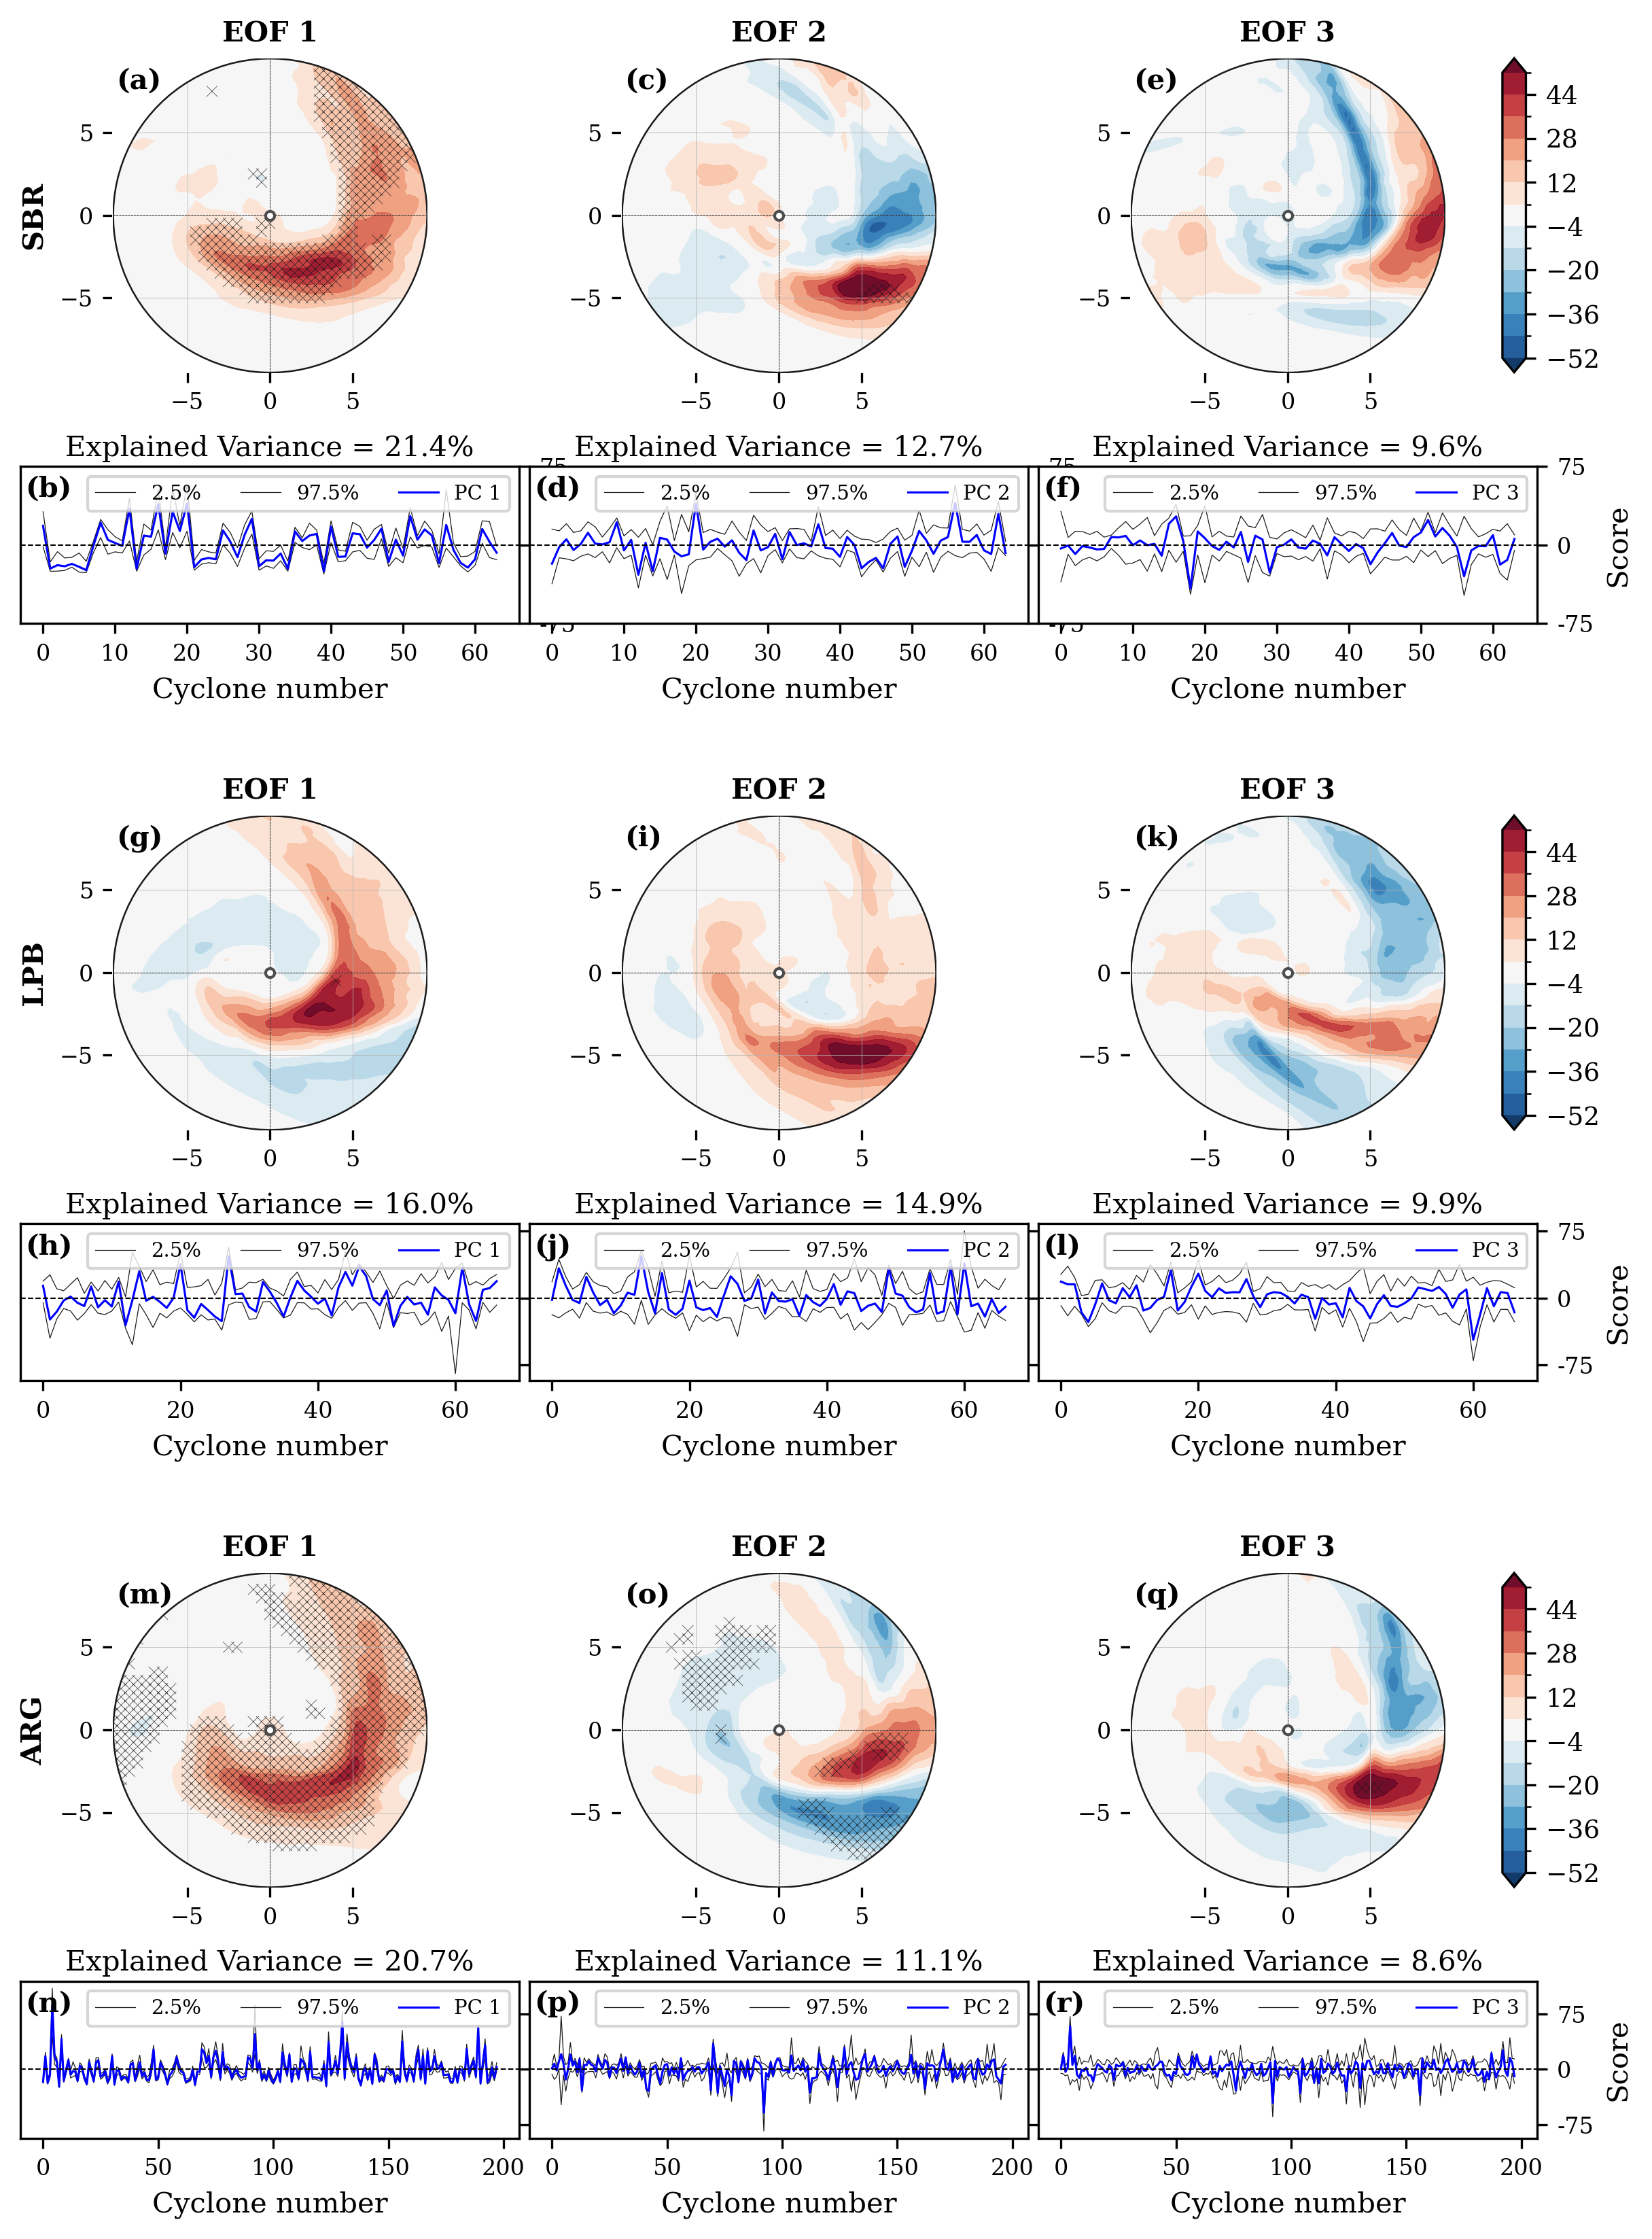
\includegraphics[width=\textwidth]{images/tp/xeof_p90_tp_mature.png}
\caption[Significancia espacial de los EOFs en fase de madurez - Subconjunto p90 (tp)]{Descomposición EOF de la precipitación total para el subconjunto extremo (p90) en fase de madurez. La disposición de paneles es idéntica a la Figura~\ref{fig:xeof_madurez_global_tp}.}
\label{fig:xeof_madurez_p90_tp}
\end{figure}

La Figura~\ref{fig:xeof_madurez_global_tp} evidencia que, para la Población Global en madurez, las áreas significativas del EOF1 se confinan al sector oriental, coherentes con el forzante WCB. A diferencia del viento, donde la significancia abarcaba dominios extensos y contiguos, aquí las zonas significativas aparecen fragmentadas, sin patrón geométrico continuo, consistente con la naturaleza discontinua de la precipitación (Sección~\ref{subsec:var_exp_tp}) \citep{oertel2021warm}. La convección embebida y los frentes estrechos generan señales localizadas pero no necesariamente coherentes a escala sinóptica.
Por el contrario, la Figura~\ref{fig:xeof_madurez_p90_tp} revela una transformación cualitativa. Consistente con el salto en varianza explicada (Sección~\ref{subsec:var_exp_tp}), el EOF1 concentra sus áreas significativas en una configuración curvada que abarca el sector sureste y sur, trazando la geometría de la banda enroscada. A diferencia de la Población Global, el achurado forma un arco continuo y denso, indicando señal estadísticamente robusta en toda la extensión de la estructura periférica. Las series de PC2 y PC3 alcanzan o superan en ciertos periodos los límites de confianza bootstrap, sugiriendo que incluso la variabilidad secundaria puede ser físicamente relevante en la madurez de los sistemas más intensos.

Esta diferencia tiene implicaciones directas para la predictibilidad de los impactos. En la Población Global, la fragmentación de la significancia indica mayor incertidumbre espacial en la ubicación de los máximos, por la variabilidad de los procesos convectivos transitorios; en los ciclones intensos durante el decaimiento, en cambio, la concentración de significancia en la banda enroscada representa una ganancia de predictibilidad geométrica, pues la huella pluviométrica se ancla en una estructura espacialmente coherente y replicable. Esto contrasta con el viento, donde la contracción de la significancia hacia el núcleo en p90 indicaba pérdida de predictibilidad para los flancos exteriores.

%%%%%%%%%%%%%%
\section{Componentes principales (PC1)}\label{sec:dinamica_pc1_tp}

La fragmentación de la varianza documentada en la madurez y su transformación hacia la coherencia en el decaimiento tienen su contraparte temporal en el comportamiento estadístico de las Componentes Principales. El contraste entre la Población Global y p90 revela una dinámica inversa a la del viento, mientras el campo cinemático mostraba un fortalecimiento progresivo de la correlación hasta la madurez seguido de un colapso en p90, el campo pluviométrico exhibe una firma correlacional invertida y distribuciones leptocúrticas en todos los estratos.

\begin{table}[htbp]
\centering
\caption[Momentos estadísticos y correlación de PC1--PC3 de precipitación - Población Global]
{Asimetría ($\gamma_1$) y curtosis ($\gamma_2$) de la PC1 de precipitación, y correlación de Spearman ($r$) entre PC1, PC2 y PC3 (con signo) y la vorticidad relativa a 850 hPa asociada a la fase (con signo, negativa en el Hemisferio Sur), para la Población Global. El signo de la correlación depende de la convención de signo de cada EOF (Sección~\ref{subsec:analisis_pc}); lo relevante es que el lado del patrón dominante en que cae cada ciclón está asociado a su intensidad. Los valores significativos ($p<0.05$) se muestran en negrita.}
\label{tab:stat_global_tp}
\begin{tabular*}{\textwidth}{@{\extracolsep{\fill}}llrrrrr}
\hline
\textbf{Región} & \textbf{Fase} & \textbf{Asimetría ($\gamma_1$)} & \textbf{Curtosis ($\gamma_2$)} & \textbf{PC1} & \textbf{PC2} & \textbf{PC3} \\
\hline
\textbf{SBR} & Incipiente       & 1.12 & 1.58 & \textbf{-0.52} & \textbf{-0.16} & \textbf{-0.26} \\
             & Intensificación & 0.85 & 0.87 & \textbf{-0.52} & \textbf{-0.13} & \textbf{0.46} \\
             & Madurez         & 1.20 & 1.53 & \textbf{0.17} & \textbf{0.65} & -0.04 \\
             & Decaimiento     & 1.49 & 2.18 & \textbf{0.19} & \textbf{0.15} & \textbf{-0.29} \\
\hline
\textbf{LPB} & Incipiente       & 1.34 & 2.85 & \textbf{-0.49} & \textbf{-0.10} & 0.07 \\
             & Intensificación & 1.03 & 1.44 & \textbf{-0.59} & -0.01 & \textbf{-0.33} \\
             & Madurez         & 1.09 & 1.45 & -0.04 & \textbf{0.61} & \textbf{-0.34} \\
             & Decaimiento     & 2.06 & 6.02 & -0.07 & \textbf{-0.24} & \textbf{-0.13} \\
\hline
\textbf{ARG} & Incipiente       & 2.55 & 9.30 & \textbf{-0.51} & \textbf{-0.18} & -0.04 \\
             & Intensificación & 1.52 & 4.06 & \textbf{-0.66} & \textbf{0.26} & \textbf{-0.22} \\
             & Madurez         & 1.74 & 5.40 & \textbf{-0.53} & \textbf{0.43} & -0.04 \\
             & Decaimiento     & 2.50 & 9.59 & \textbf{-0.25} & 0.00 & \textbf{0.13} \\
\hline
\end{tabular*}
\end{table}


\subsection{Población Global}\label{subsec:pc1_global_tp}

La Tabla~\ref{tab:stat_global_tp} documenta asimetría, curtosis y correlación de Pearson de la PC1 con la vorticidad mínima a 850~hPa para la Población Global, desagregadas por región y fase.

El análisis de los momentos estadísticos revela una característica distintiva, la presencia persistente de colas pesadas (leptocurtosis positiva) a lo largo de todo el ciclo de vida. A diferencia del viento, donde la curtosis evolucionaba hacia valores cercanos a cero o negativos en la madurez, aquí se observan valores de $\gamma_2$ positivos en las tres regiones: SBR oscila entre $+0.87$ (intensificación) y $+2.18$ (decaimiento); LPB exhibe curtosis pronunciada en incipiencia ($+2.85$) y decaimiento ($+6.02$); ARG presenta los valores más extremos, superiores a $+9$ tanto en incipiencia como en decaimiento. El sesgo positivo persistente ($\gamma_1 > +0.8$ en la mayoría de los casos) refleja la presencia de eventos con anomalías pluviométricas intensas respecto al patrón medio.

El examen de las correlaciones entre PC1 y vorticidad revela un desacoplamiento progresivo durante la madurez en las regiones oceánicas. En SBR, la correlación negativa moderada de las fases iniciales ($\rho \approx -0.52$) invierte su signo en madurez ($\rho = +0.17$, significativo) y decaimiento ($\rho = +0.19$, significativo). LPB muestra un patrón similar. Correlaciones negativas significativas durante el desarrollo ($\rho = -0.49$ en incipiencia, $-0.59$ en intensificación) que colapsan a valores no significativos en madurez ($\rho = -0.04$, $p = 0.26$) y decaimiento ($\rho = -0.07$, $p = 0.07$). ARG mantiene correlaciones negativas significativas durante todo el ciclo, con un fortalecimiento inicial hacia la intensificación ($-0.66$) y un debilitamiento posterior hasta el decaimiento ($-0.25$).

Este comportamiento refleja procesos físicos diferenciados. El cambio de signo en SBR y el colapso en LPB durante la madurez responden a la divergencia entre intensidad dinámica y actividad convectiva ya documentada. En estas regiones, los sistemas que alcanzan vorticidad extrema ocluyen rápidamente, y la intrusión seca suprime la convección profunda en el dominio central lagrangiano; por ello la PC1 deja de escalar negativamente con la intensidad del vórtice como en las fases tempranas, y el débil vínculo positivo que emerge en madurez y decaimiento ($\rho \approx +0.17$ a $+0.19$) sugiere que la amplitud del modo pasa a depender de la banda periférica y no de la intensidad dinámica, pues los ciclones p90 presentan anomalías menores en el núcleo al secarse este. En ARG, consistente con las oclusiones más lentas y el control orográfico ya señalados (Sección~\ref{sec:pdf_tp}), el agotamiento de humedad es más gradual, manteniendo un acoplamiento residual entre vorticidad y precipitación por más tiempo.

La variabilidad temporal de estas series de PC1, manifestada en picos de amplitud interanual, responde además a fluctuaciones de gran escala en la circulación hemisférica. Las oscilaciones de baja frecuencia en la baroclinicidad del Hemisferio Sur \citep{machado2020influence} modulan la posición e intensidad de los sistemas ciclónicos, afectando indirectamente su capacidad de generar precipitación, de modo que en periodos de mayor inestabilidad baroclínica la PC1 exhibe amplitudes superiores a la media.

\begin{table}[htbp]
\centering
\caption[Momentos estadísticos y correlación de PC1--PC3 de precipitación - Subconjunto p90]
{Asimetría ($\gamma_1$) y curtosis ($\gamma_2$) de la PC1 de precipitación, y correlación de Spearman ($r$) entre PC1, PC2 y PC3 (con signo) y la vorticidad relativa a 850 hPa asociada a la fase (con signo, negativa en el Hemisferio Sur), para el subconjunto extremo (p90). El signo de la correlación depende de la convención de signo de cada EOF (Sección~\ref{subsec:analisis_pc}); lo relevante es que el lado del patrón dominante en que cae cada ciclón está asociado a su intensidad. Los valores significativos ($p<0.05$) se muestran en negrita.}
\label{tab:stat_p90_tp}
\begin{tabular*}{\textwidth}{@{\extracolsep{\fill}}llrrrrr}
\hline
\textbf{Región} & \textbf{Fase} & \textbf{Asimetría ($\gamma_1$)} & \textbf{Curtosis ($\gamma_2$)} & \textbf{PC1} & \textbf{PC2} & \textbf{PC3} \\
\hline
\textbf{SBR} & Incipiente       & 1.57 & 3.48  & \textbf{-0.36} & \textbf{-0.53} & -0.22 \\
             & Intensificación & 1.20 & 1.67  & \textbf{-0.48} & \textbf{-0.43} & -0.24 \\
             & Madurez         & 0.41 & -0.67 & -0.17 & -0.22 & -0.11 \\
             & Decaimiento     & 4.02 & 19.77 & \textbf{-0.34} & 0.17 & -0.18 \\
\hline
\textbf{LPB} & Incipiente       & 1.90 & 4.52  & \textbf{-0.49} & \textbf{-0.31} & 0.22 \\
             & Intensificación & 0.60 & -0.38 & \textbf{-0.43} & -0.01 & \textbf{0.26} \\
             & Madurez         & 0.56 & 0.16  & -0.03 & -0.18 & 0.02 \\
             & Decaimiento     & 4.34 & 23.18 & \textbf{-0.50} & 0.09 & 0.03 \\
\hline
\textbf{ARG} & Incipiente       & 4.43 & 30.88 & \textbf{-0.44} & \textbf{-0.29} & \textbf{-0.23} \\
             & Intensificación & 1.87 & 5.15  & \textbf{-0.37} & \textbf{0.21} & \textbf{-0.28} \\
             & Madurez         & 1.66 & 4.53  & \textbf{-0.24} & 0.03 & -0.14 \\
             & Decaimiento     & 1.96 & 3.37  & \textbf{-0.39} & \textbf{0.32} & 0.10 \\
\hline
\end{tabular*}
\end{table}


\subsection{Subconjunto (p90)}\label{subsec:pc1_p90_tp}

La Tabla~\ref{tab:stat_p90_tp} expone los parámetros estadísticos y correlaciones para el subconjunto extremo. A diferencia de la leptocurtosis persistente de la Población Global, aquí se documenta una evolución no monotónica hacia valores extremos en el decaimiento, junto con un colapso sistemático de las correlaciones en la madurez.

El análisis de las distribuciones revela una heterogeneización dramática. En SBR se observa leptocurtosis marcada en las fases iniciales ($\gamma_2 = +3.48$ en incipiencia, $+1.67$ en intensificación), seguida de un colapso a distribución cuasi-normal en madurez ($\gamma_2 = -0.67$) y una explosión leptocúrtica en decaimiento ($\gamma_2 = +19.77$, $\gamma_1 = +4.02$). LPB reproduce este patrón con valores aún más extremos: curtosis de $+4.52$ en incipiencia, simetría en madurez ($\gamma_2 = +0.16$) y valores superiores a $+23$ en decaimiento. ARG presenta la curtosis más elevada del conjunto en incipiencia ($\gamma_2 = +30.88$), manteniendo valores positivos extremos durante todo el ciclo. En ARG, esta curtosis extrema en incipiencia es consistente con la mayor heterogeneidad estructural que caracteriza a esta fase (Sección~\ref{subsec:tb_fases}), acentuada por un mecanismo de génesis a sotavento de los Andes (Sección~\ref{subsec:tb_arg}), más variable que el forzamiento termodinámico oceánico que organiza la génesis en SBR y LPB. La mayoría de los sistemas incipientes de ARG proyecta débilmente sobre el EOF1, mientras que unos pocos casos, alineados por azar con la geometría del modo dominante, generan la cola pesada que eleva la curtosis observada.

Las correlaciones con la vorticidad colapsan durante la madurez en SBR ($\rho = -0.17$, no significativo) y LPB ($\rho = -0.03$, $p = 0.80$), recuperándose en el decaimiento ($-0.34$ y $-0.50$ respectivamente), mientras ARG mantiene valores negativos significativos aunque atenuados ($-0.24$ en madurez).

El colapso correlacional en SBR y LPB durante la madurez es el correlato temporal del desacoplamiento espacial documentado en las secciones previas, ya que una vez consolidada la banda enroscada, la amplitud de la PC1 ya no depende de la profundidad del vórtice, sino de cuánto de esa banda permanece dentro del dominio lagrangiano a medida que el ciclón se disipa, lo que explica la evolución hacia la normalidad estadística en madurez seguida de la explosión leptocúrtica en decaimiento.

La persistencia de correlaciones significativas en ARG durante toda la evolución es consistente con el control orográfico
andino y las oclusiones más lentas ya señalados (Sección~\ref{subsec:pc1_global_tp}), lo que sostendría un acoplamiento más persistente entre vorticidad y precipitación, aunque atenuado respecto a las fases iniciales.
Estos resultados demuestran que el campo de precipitación es estructuralmente más complejo que el cinemático. La combinación de distribuciones cambiantes, correlaciones que colapsan y recuperan, y diferencias regionales marcadas indica que parametrizar la precipitación usando únicamente la vorticidad resulta inadecuado durante la fase crítica de madurez en las regiones oceánicas, donde el desacoplamiento es más pronunciado.

\section{Síntesis}\label{sec:sintesis_tp}

El análisis del campo de precipitación total muestra que la arquitectura pluviométrica evoluciona desde un régimen de dispersión frontal hacia uno de concentración ocluida, según la intensidad dinámica del sistema.

En la Población Global, SBR y LPB muestran perfiles anchos y planos con pico modal entre 10 y 20~mm/h; ARG concentra su pico en valores bajos ($\sim$5--10~mm/h). En el subconjunto p90, la separación respecto al global es clara durante la intensificación (colas hasta 60~mm/h en SBR y LPB), pero se invierte en madurez y decaimiento. La curva p90 colapsa hacia magnitudes mínimas (1--4~mm/h, densidad $>$0.17 en SBR), mientras la Población Global retiene perfiles amplios centrados en 15--20~mm/h. Este colapso modal, ausente en el campo de viento, evidencia que la intensidad dinámica y la magnitud pluviométrica se desacoplan progresivamente a medida que el ciclón madura.

En la Población Global, los máximos se organizan con asimetría persistente hacia el sector oriental y sureste, firma del WCB, con densidades máximas de $\sim$29$\times10^{-4}$ en SBR durante la intensificación. En el subconjunto p90, esta organización se reconfigura drásticamente al alcanzar la madurez. Los máximos se alejan del centro de vorticidad y se confinan en bandas estrechas y arqueadas (\textit{wrap-around precipitation}), producto de la intrusión seca asociada al modelo de Shapiro-Keyser. En el decaimiento, esta banda persiste anclada al flanco sureste y oriental (SBR: $\sim$7$\times10^{-4}$ en el borde del dominio; LPB: elongación este hasta $+7^{\circ}$), mientras en la Población Global la señal se difumina.
En la Población Global, la varianza espacial se distribuye entre múltiples modos, con el EOF1 explicando solo entre 11.1\% y 16.4\% de la varianza total, reflejo de la naturaleza discontinua e intermitente de la precipitación.
En el subconjunto p90, el EOF1 se concentra abruptamente durante madurez y decaimiento, alcanzando su máximo en LPB (36.5\% en decaimiento, $+$22.2 puntos respecto al global) y valores comparables en SBR (26.2\% en decaimiento).
Este salto, sin equivalente en el campo de viento, responde a la consolidación de la banda enroscada como estructura espacialmente coherente y cuasi-estacionaria.

En la Población Global, la correlación entre PC1 y la vorticidad mínima es débil o negativa en las fases iniciales
($\rho \approx -0.5$), pero diverge regionalmente hacia la madurez: se invierte a positiva y significativa en SBR,
colapsa a no significativa en LPB, y se mantiene negativa aunque atenuada en ARG.
En el subconjunto p90, el acoplamiento colapsa durante la madurez en SBR ($\rho = -0.17$, no significativo) y LPB ($\rho = -0.03$, $p = 0.80$), recuperándose parcialmente en el decaimiento ($-0.34$ y $-0.50$, respectivamente); ARG mantiene correlaciones significativas aunque atenuadas durante todo el ciclo ($-0.24$ en madurez).
Esto confirma que, en las regiones oceánicas, la organización espacial de la precipitación extrema deja de depender linealmente de la intensidad rotacional del vórtice una vez que la oclusión desacopla el núcleo dinámico de la fuente de humedad.
En conjunto, estos resultados muestran que, mientras el campo de viento se hiperconcentra espacialmente al alcanzar la madurez (Capítulo~\ref{cap:resultados_wind10}), el campo de precipitación experimenta el proceso inverso en su núcleo central. La intrusión seca vacía de humedad al centro del sistema y desplaza la actividad pluviométrica hacia una banda periférica arqueada. En los ciclones más intensos, el forzante eólico se concentra en el cuadrante noroeste (cinta transportadora fría) mientras el remanente pluviométrico se organiza en el cuadrante sureste y sur (banda enroscada), configurando una separación espacial sistemática entre los forzantes cinemático e hidrológico del sistema.

Las diferencias regionales modulan esta arquitectura mediante la interacción con las condiciones de superficie. En SBR y LPB, los flujos de calor latente oceánico y el SALLJ favorecen el desacople más pronunciado entre vorticidad y precipitación, mientras que en ARG la modulación orográfica y las oclusiones más lentas generan un régimen de transición más gradual entre dinámica y humedad, como refleja la persistencia de correlaciones significativas en esta región.
Esta base empírica sobre la precipitación, en particular la descripción del desacople por fases entre viento y lluvia, provee el cimiento para el análisis combinado mediante EOF multivariado (MEOF; Sección~\ref{subsec:eof_multivariado}) en el capítulo siguiente, donde la covarianza conjunta de ambos campos se sintetiza en los prototipos estructurales descritos en la Sección~\ref{subsec:prototipos}.
